\documentclass{beamer}

\mode<presentation>
{

  \usetheme{Boadilla}
  \usecolortheme{whale}
  \setbeamercovered{transparent}
  
  \setbeamertemplate{footline}[frame number]{}
  \setbeamertemplate{navigation symbols}{}

}

\usepackage[english]{babel}
\usepackage[utf8]{inputenc}
\usepackage{times}
\usepackage[T1]{fontenc}

\usepackage{amsmath, amsthm, amssymb, amsfonts}
\usepackage{mathtools}

\usepackage{graphicx}


\usepackage{natbib}
\bibliographystyle{unsrtnat}

\usepackage{float}
\usepackage{bbm}
\usepackage{mathrsfs}

% ======== Alix notation =======
\def\th{\theta}
\def\eps{\epsilon}
\def\beq{\begin{equation}}
\def\eeq{\end{equation}}
\def\bdm{\begin{displaymath}}
\def\edm{\end{displaymath}}
\def\vsd{\vspace{0.1in}}
% ==============================

\usepackage{listings}
\usepackage{relsize}



\title{Take Me Out to (Analyze) the Ballgame}
\subtitle{Visualization and Analysis Techniques for Big Spatial Data}
\author{Chris Comiskey} 
\institute{Oregon State University} 
\date{\today} 

% Delete this, if you do not want the table of contents to pop up at the beginning of each subsection:

\AtBeginSection[]
{
 \begin{frame}<beamer>{Outline}
   \tableofcontents[currentsection,currentsubsection]
 \end{frame}
}

\AtBeginSubsection[]
{
 \begin{frame}<beamer>{Outline}
   \tableofcontents[currentsection,currentsubsection]
 \end{frame}
}

\begin{document}

\begin{frame}
  \titlepage
\end{frame}

\begin{frame}{Baseball, Baseball, Baseball} % ==================
\begin{columns}

\column{0.5\textwidth}

\begin{itemize}
\item Chris, rookie year
\end{itemize}
        \begin{figure}[H]
      	\centering
      	\includegraphics[scale=.65]{Images/CWC_Royals.pdf}
      	\end{figure}

\column{0.5\textwidth}

\begin{itemize}
\item Chris, Boston Red Sox
\end{itemize}
  \begin{figure}[H]
	\centering
	\includegraphics[scale=.3]{Images/RedSox.jpg}
	\end{figure}

\end{columns}
\end{frame}

\begin{frame}{Hitting Analytics} % ==================
\begin{columns}
\column{0.5\textwidth}
\begin{itemize}
\item $\text{``The Science of Hitting''}_{\text{1970}}$
\end{itemize}

        \begin{figure}[H]
      	\centering
      	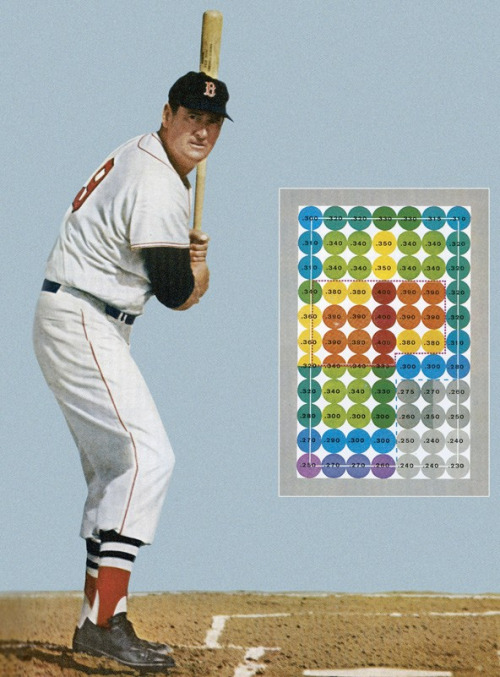
\includegraphics[scale=.22]{Images/Williams.jpg}
      	\end{figure}

\begin{itemize}
\item Iconic breakthrough, hitter
\item No data
\end{itemize}

\column{0.5\textwidth}
\begin{itemize}
\item The Statistics of Hitting
\end{itemize}
  \begin{figure}[H]
	\centering
	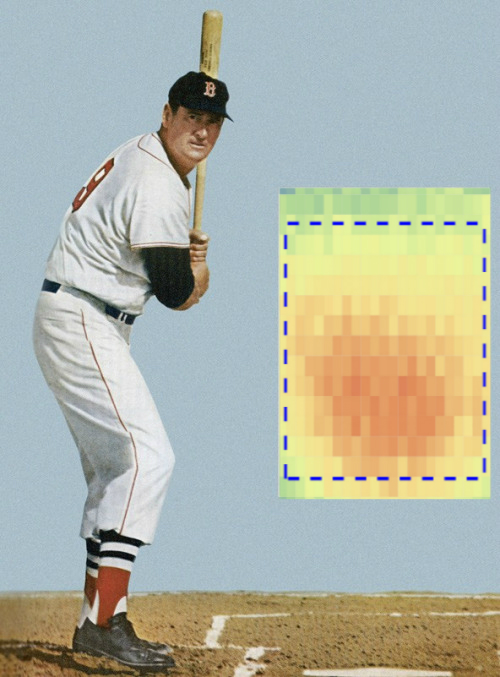
\includegraphics[scale=.22]{Images/WilliamsMother.jpg}
	\end{figure}
\begin{itemize}
\item PITCHf/x data, R, heat maps
\item SGLMMs, Stan, PPMs, INLA
\end{itemize}

\end{columns}
\end{frame}

\section{Variable-Resolution Heat Maps}

\begin{frame}{Empirical Success Probability Heat Map} % =============
\begin{columns}

\column{0.5\textwidth}

  \begin{figure}[H]
	\centering
	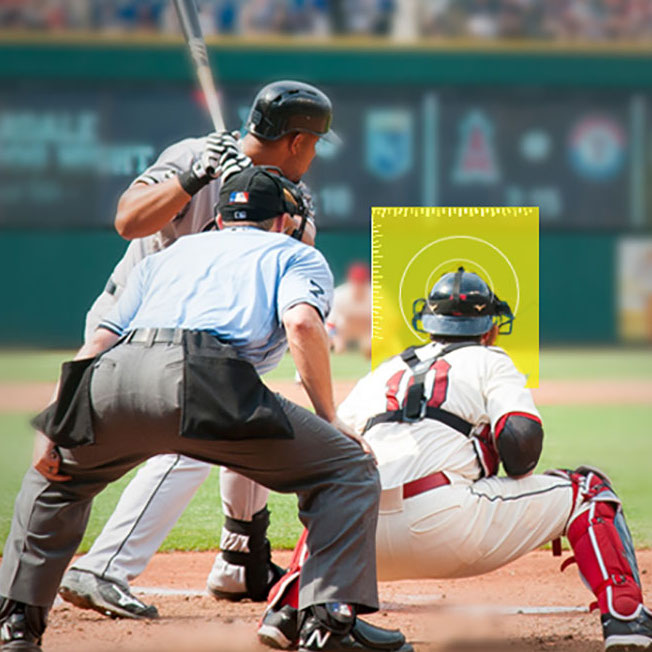
\includegraphics[scale=.26]{Images/StrikeZone3.jpg}
	\end{figure}

\column{0.5\textwidth}
  \begin{figure}[H]
	\centering
	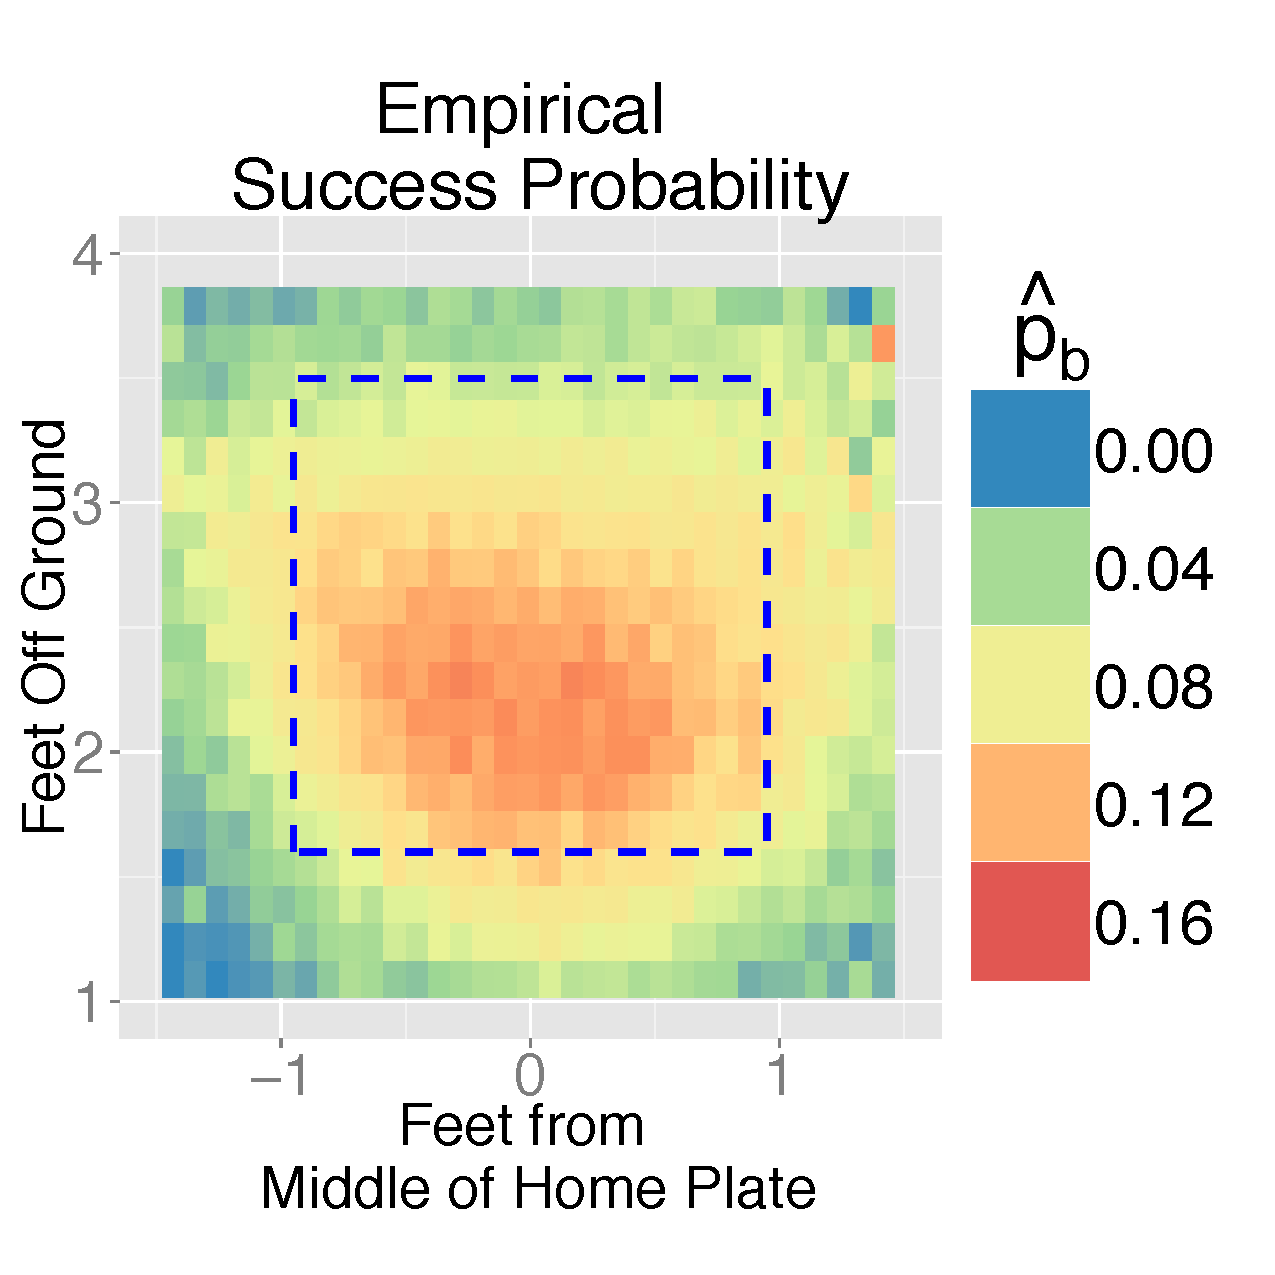
\includegraphics[scale=.07]{Images/Mothership.jpg}
	\end{figure}

\end{columns}
\end{frame}

\begin{frame}{Empirical Success Probability Heat Map} % ====

\begin{itemize}
\addtolength{\itemsep}{0.5\baselineskip}
\item Swings: $i = 1,2,\ldots, N$
\item $\text{Bernoulli}(\pi_{i})$ trials:
    \bdm
    S_i = \left\{\begin{array}{ll} 1; & \mbox{swing success} \\
    					 0; & \mbox{swing failure} \\ \end{array} \right.
    \edm
\item Location $(x_i,y_i)$
\item Grid boxes $G_1,G_2,\ldots,G_B$
\item Box $b$ totals:
    \bdm
    N_b = \sum_{i=1}^N I_{(x_i,y_i) \in G_b}
    \edm
\item Box $b$ empirical success:
    \bdm
     p_b = \frac{1}{N_b} \sum_{i=1}^N S_i I_{(x_i,y_i) \in G_b}
    \edm
\end{itemize}
\end{frame}

\begin{frame}{Heat Map Resolution Selection}{Jhonny Peralta}
  \begin{figure}[H]
	\centering
	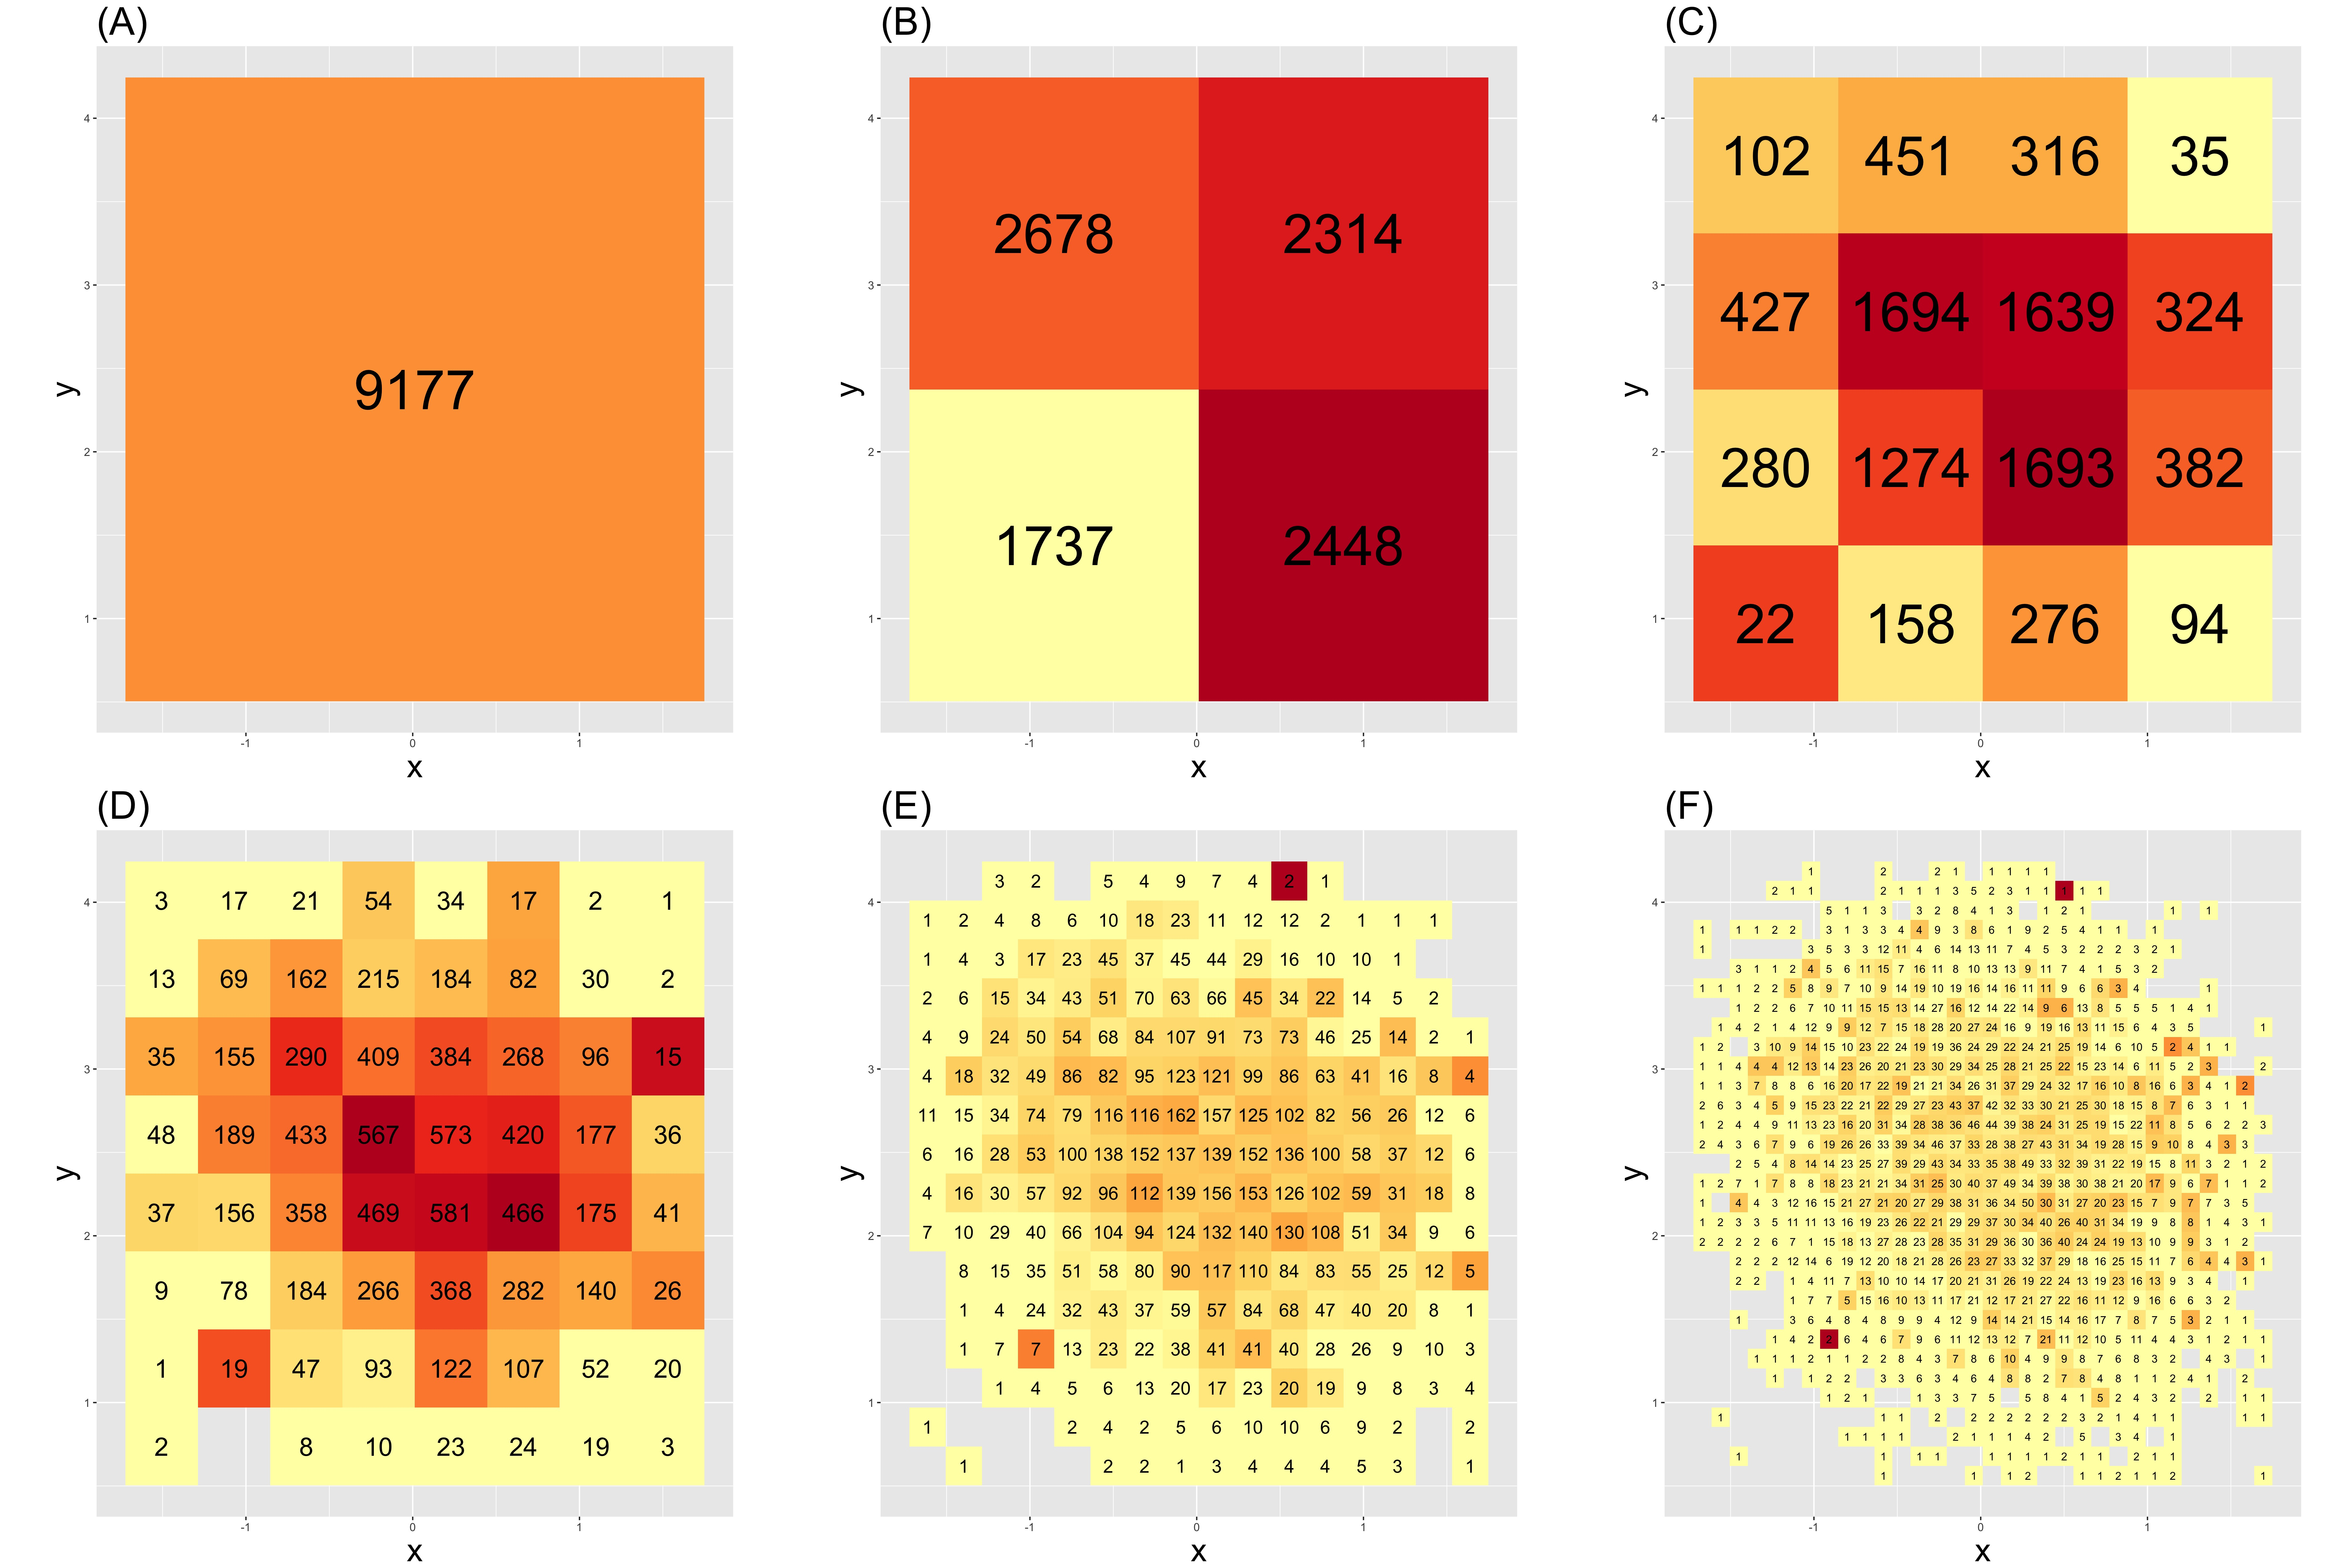
\includegraphics[scale=.0425]{Images/Chapter_VarRes.jpg}
	\end{figure}
\end{frame}

\begin{frame}{A Thing of Beauty}{}
  \begin{figure}[H]
	\centering
	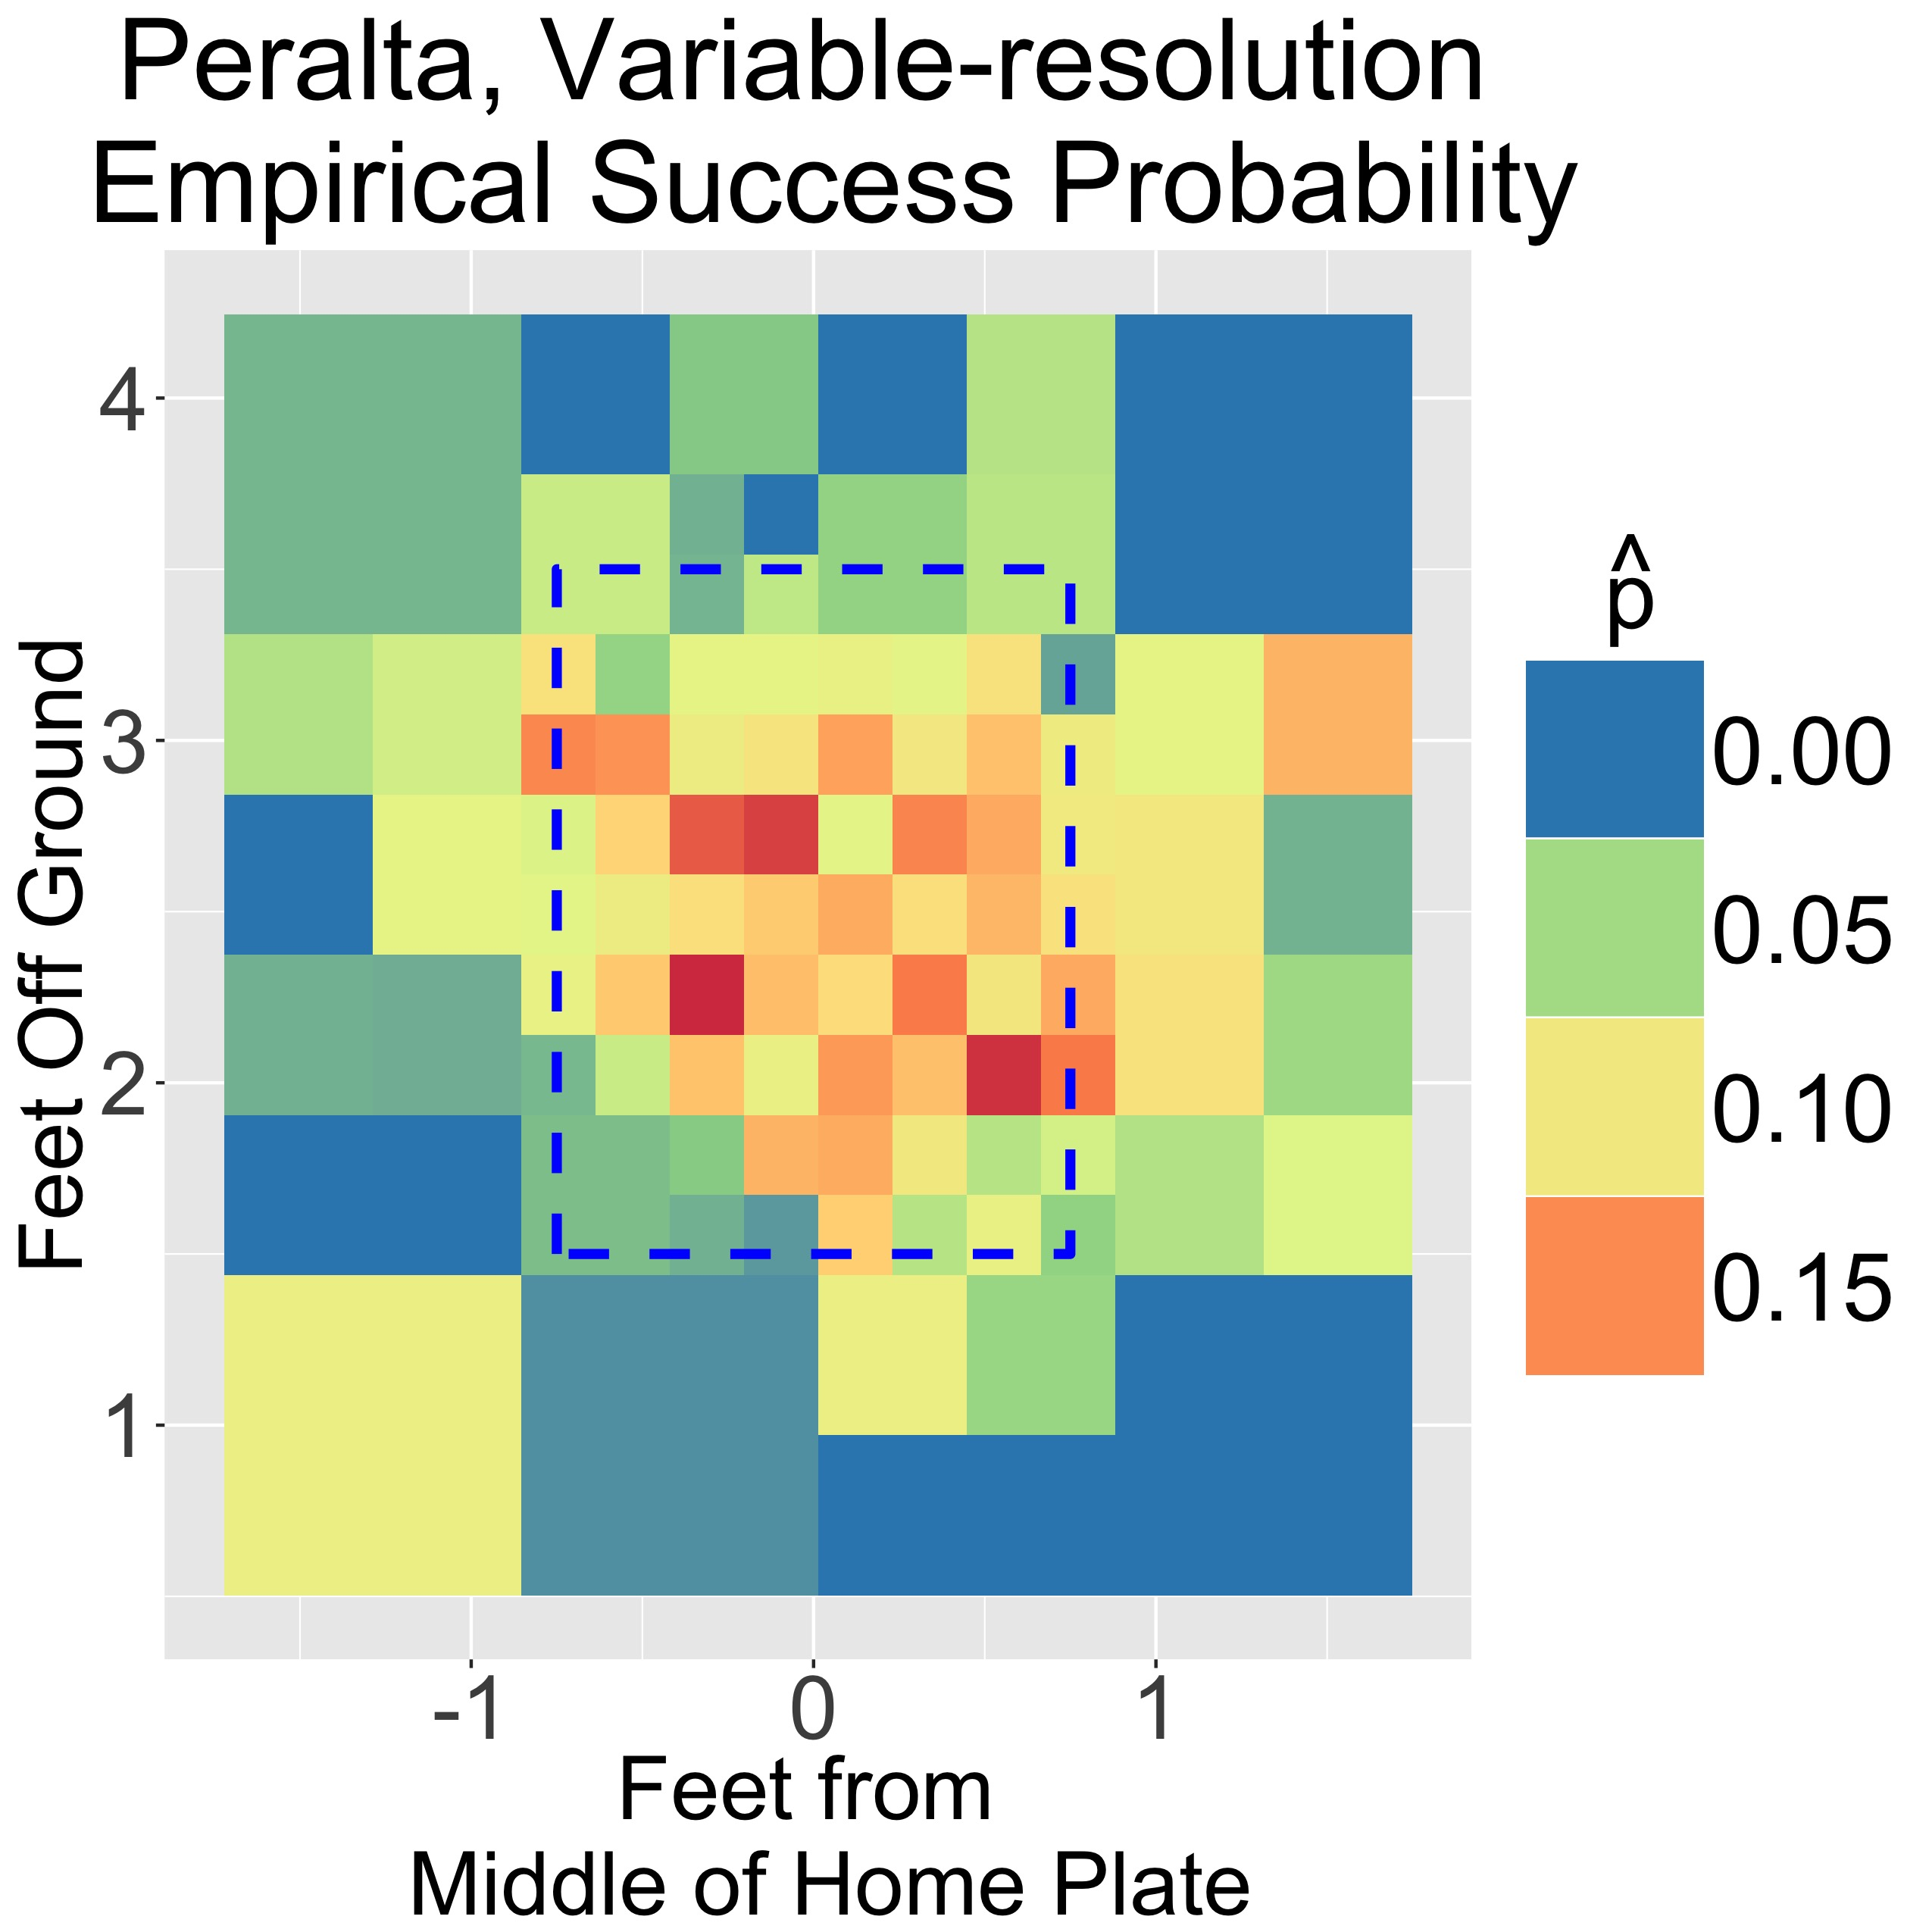
\includegraphics[scale=.075]{Images/Peralta_var-res.jpg}
	\label{fig:interp}
  \end{figure}
\end{frame}

\begin{frame}{Variable-Resolution Heat Maps}{Jhonny Peralta}
\begin{itemize}
\item Stopping rule
\item Subdivision method
\item VR algorithm
\end{itemize}
  \begin{figure}[H]
	\centering
	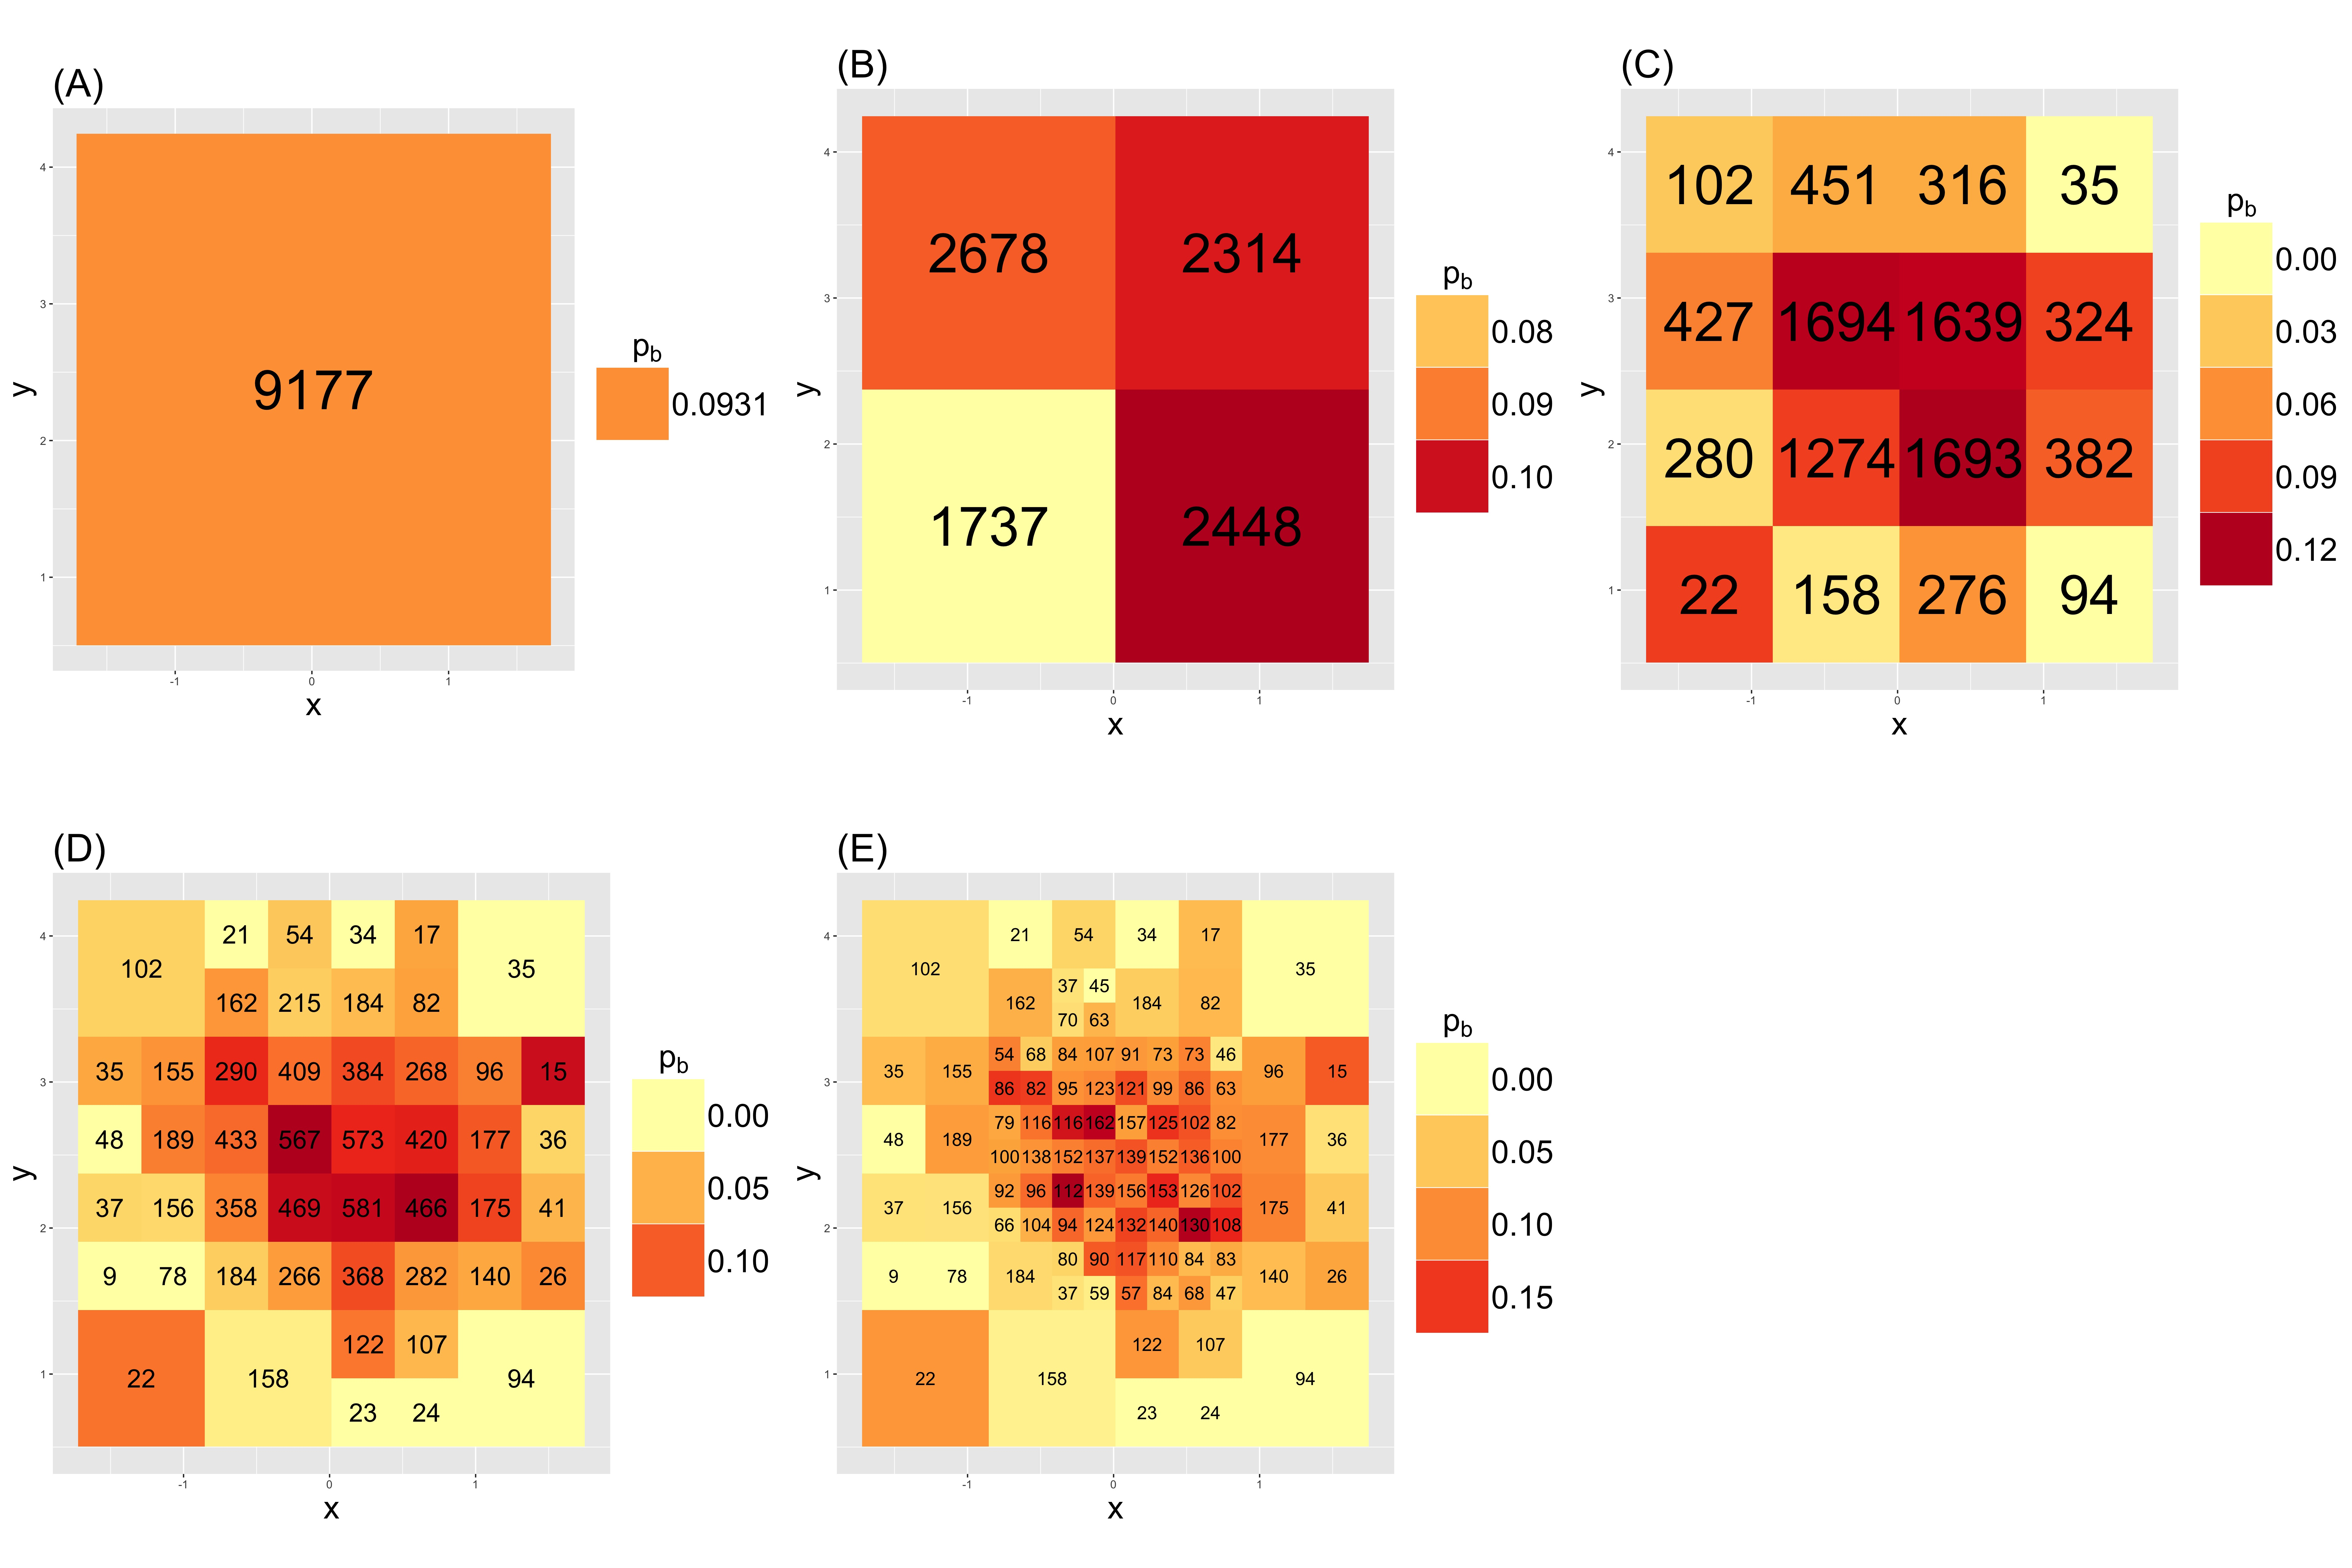
\includegraphics[scale=.036]{Images/6_200.jpg}
	\end{figure}
\end{frame}

\begin{frame}{Variable-Resolution Heat Maps}{Combine Resolutions}
\begin{itemize}
\addtolength{\itemsep}{0.5\baselineskip}
\item Stopping rule: sample size threshold
\item Combine resolutions
\item Resolution conveys data density
\item Improvements:
  \begin{itemize}
  \addtolength{\itemsep}{0.5\baselineskip}
  \item Subdivision methods
  \item Subdivision criteria
  \end{itemize}
\end{itemize}
\end{frame}

\begin{frame}{varyres(...) in {\bf varyres}}
  \begin{figure}[H]
	\centering
	\includegraphics[scale=.35]{Images/varyres.png}
	\end{figure}
	\end{frame}

\section{Interactive Heat Map Confidence Intervals}

\begin{frame}{Generalized Linear Model}{}
$$Y_{i}|\mathbf{X}_{i}(\mathbf{s}_{i}) \stackrel{ind}{\sim} \mbox{Bernoulli}(\pi_{i}) $$
$$ \text{logit}(\pi_{i}|\pmb{s}_{i}) = \mathbf{X}_{i}(\mathbf{s}_{i})\pmb{\beta} $$
\begin{itemize}
  \addtolength{\itemsep}{0.5\baselineskip}
\item Swings: $i = 1,2,\ldots, N$
\item Pitch location: $\mathbf{s}_{i} = (x_{i},y_{i})$
\item Biomechanical covariates: $\mathbf{X}_{i}(\mathbf{s}_{i})$
\item Fit to Jhonny Peralta data
\end{itemize}

\end{frame}

\begin{frame}{Logistic Regression Model}{Jhonny Peralta} % ======
$$Y_{i}|\mathbf{X}_{i}(\mathbf{s}_{i}) \stackrel{ind}{\sim} \mbox{Bernoulli}(\pi_{i}) $$
$$ \text{logit}(\pi_{i}|\pmb{s}_{i}) = \mathbf{X}_{i}(\mathbf{s}_{i})\pmb{\beta}, $$
  \begin{figure}[H]
	\centering
	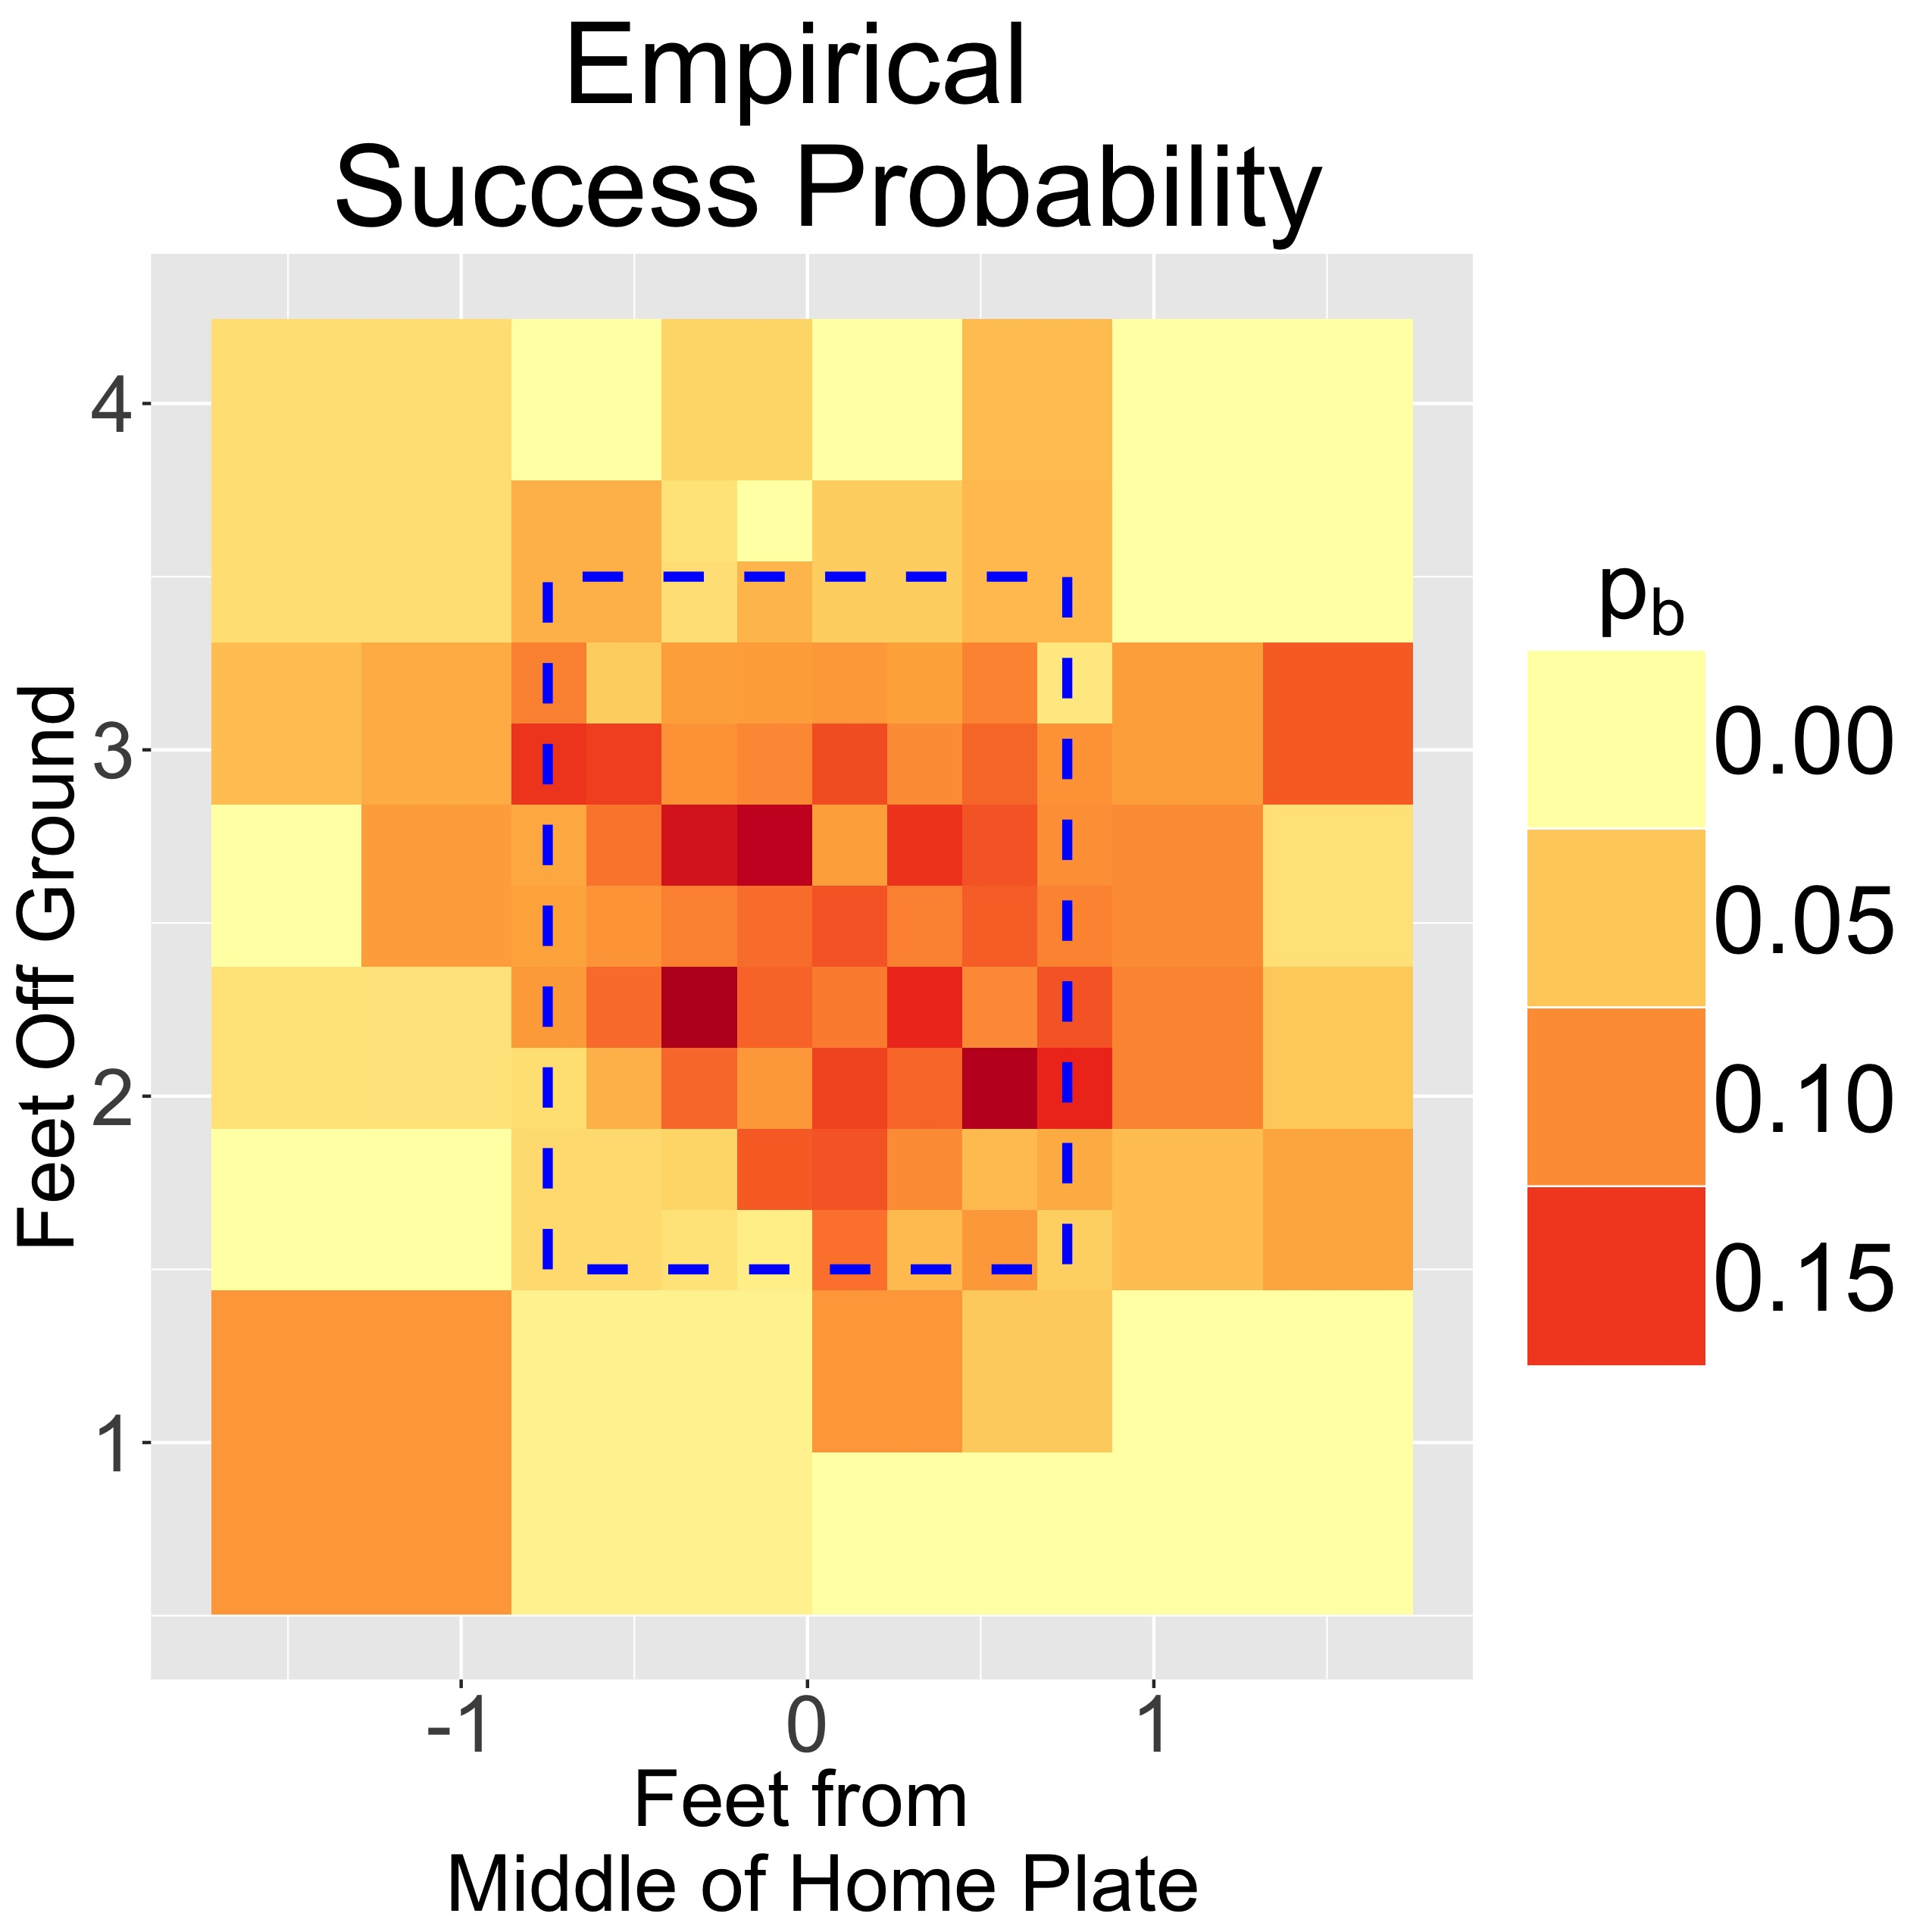
\includegraphics[scale=.055]{Images/Peralta_var-res2.jpg}
	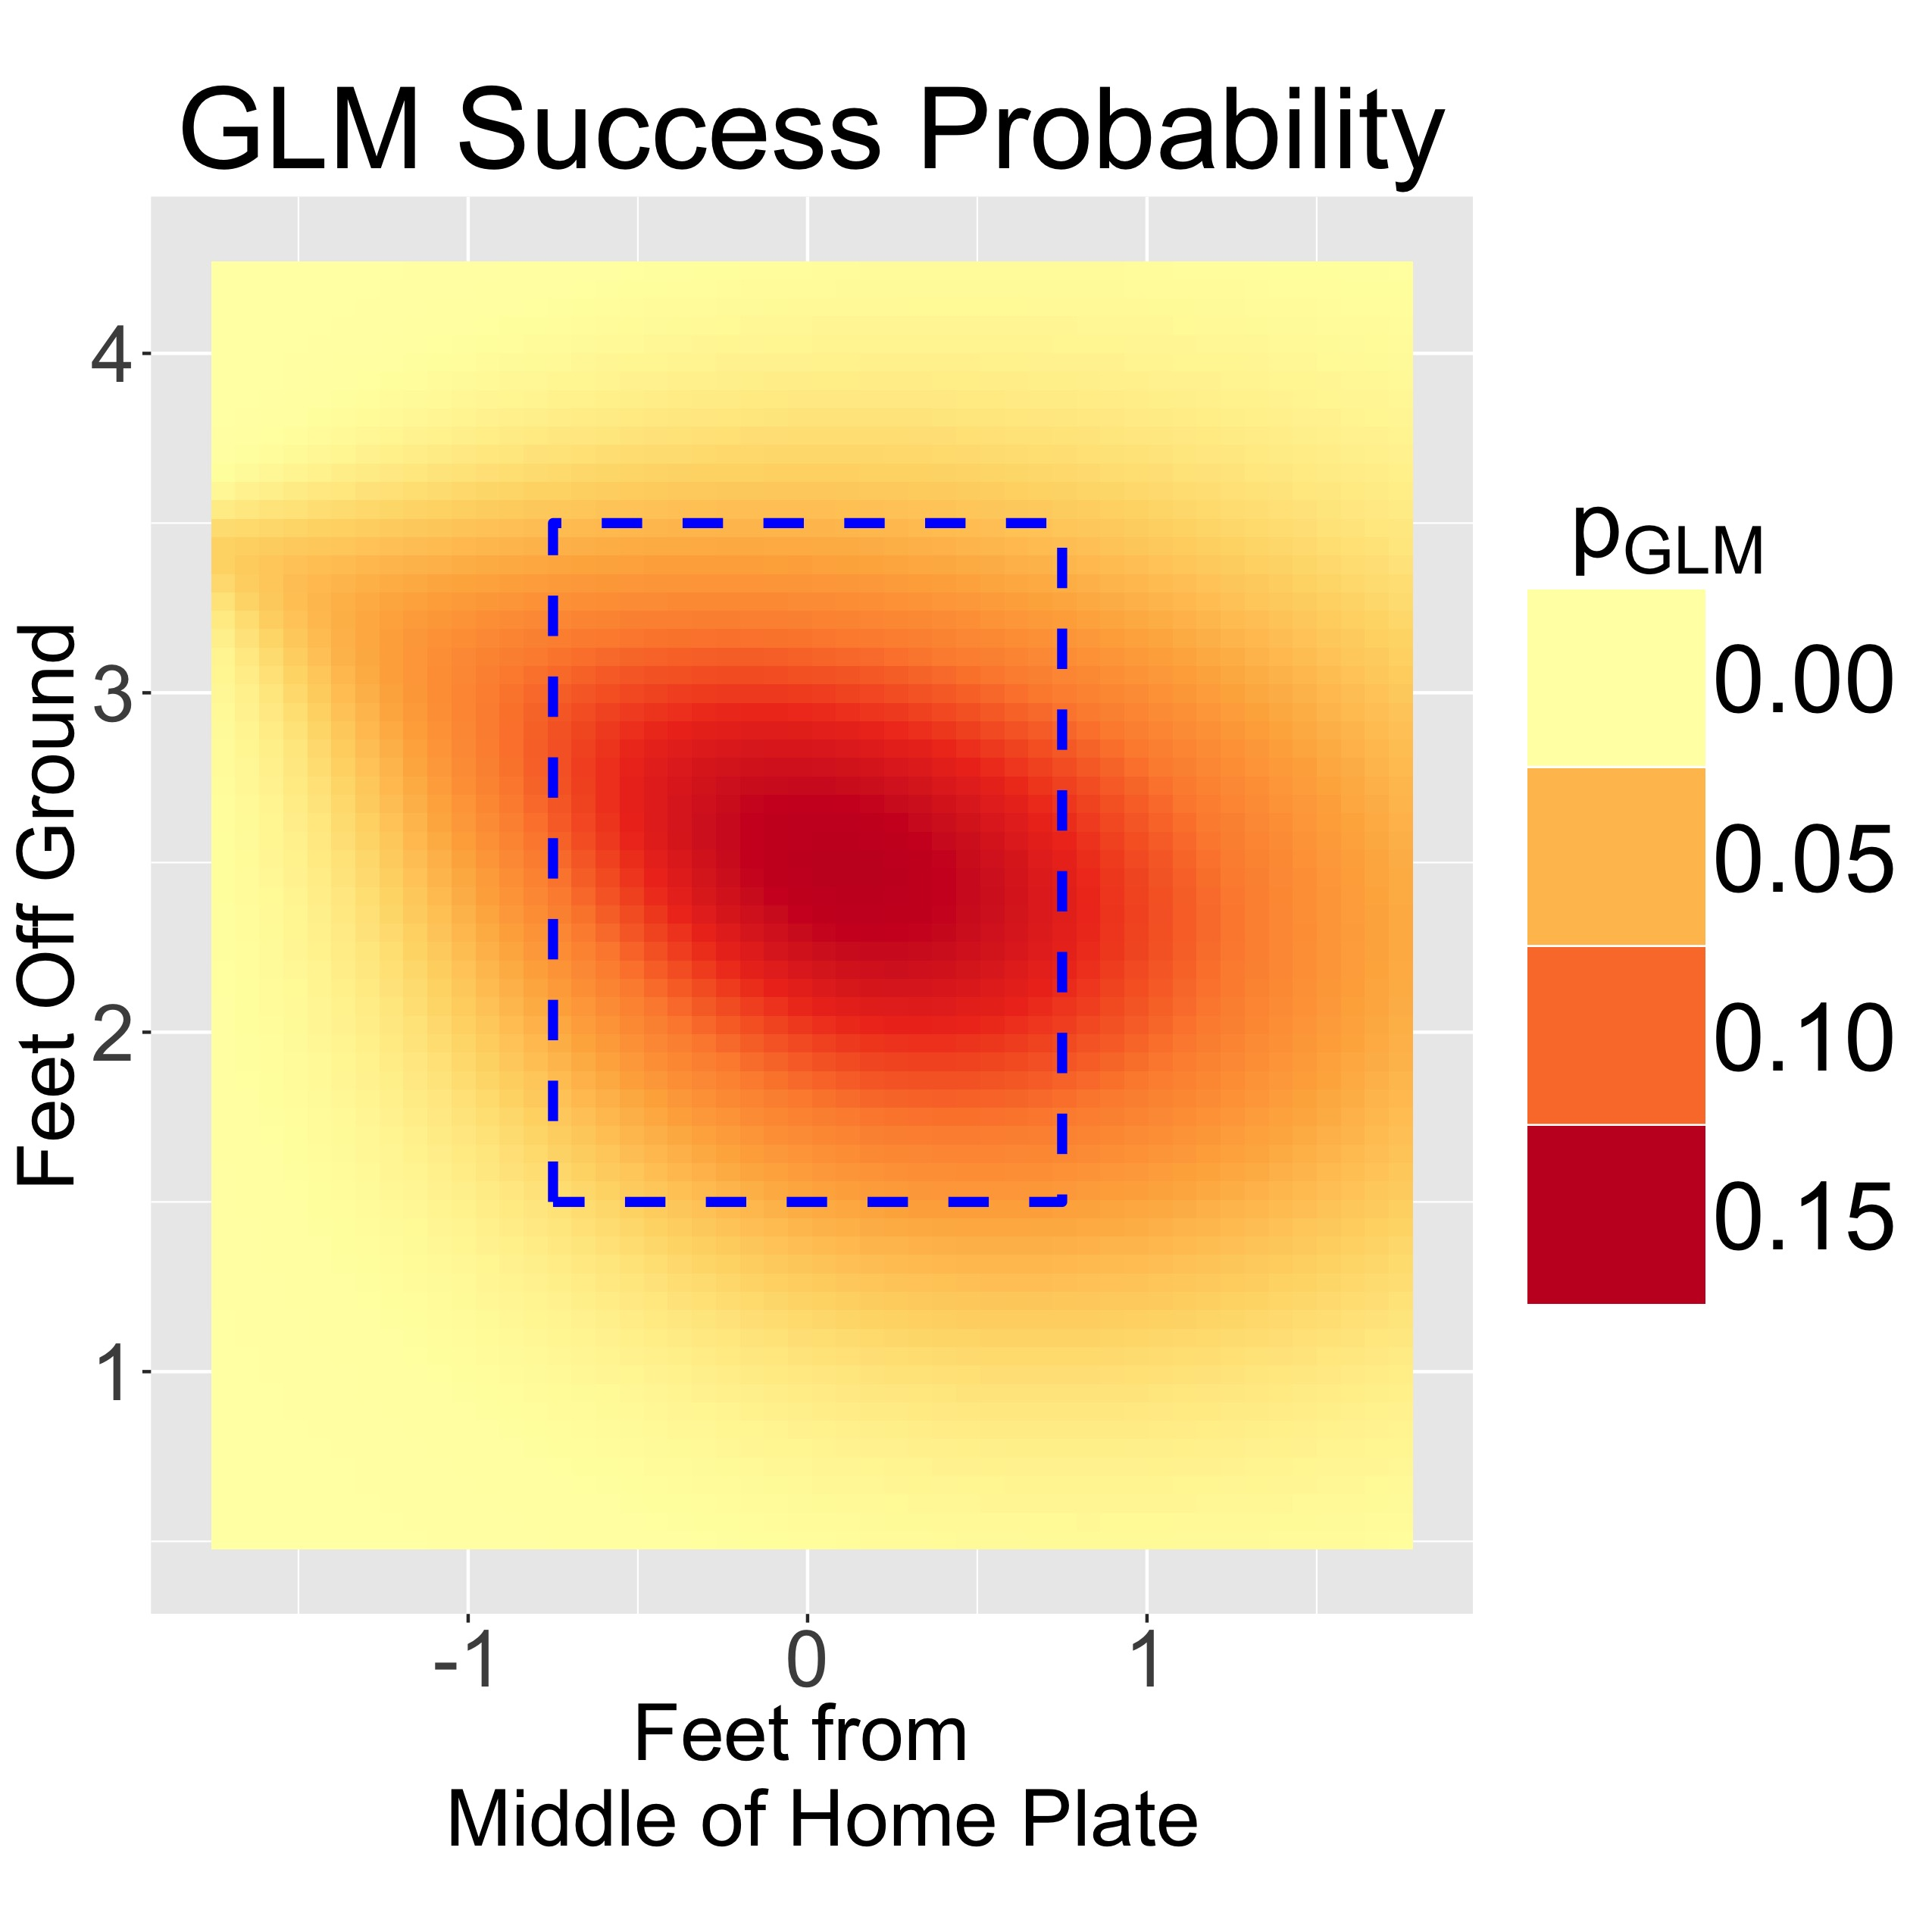
\includegraphics[scale=.055]{Images/Peralta_fit.jpg}
	\end{figure}
\end{frame}

\begin{frame}{Logistic Regression Model}{Jhonny Peralta} % ======
  \begin{figure}[H]
	\centering
	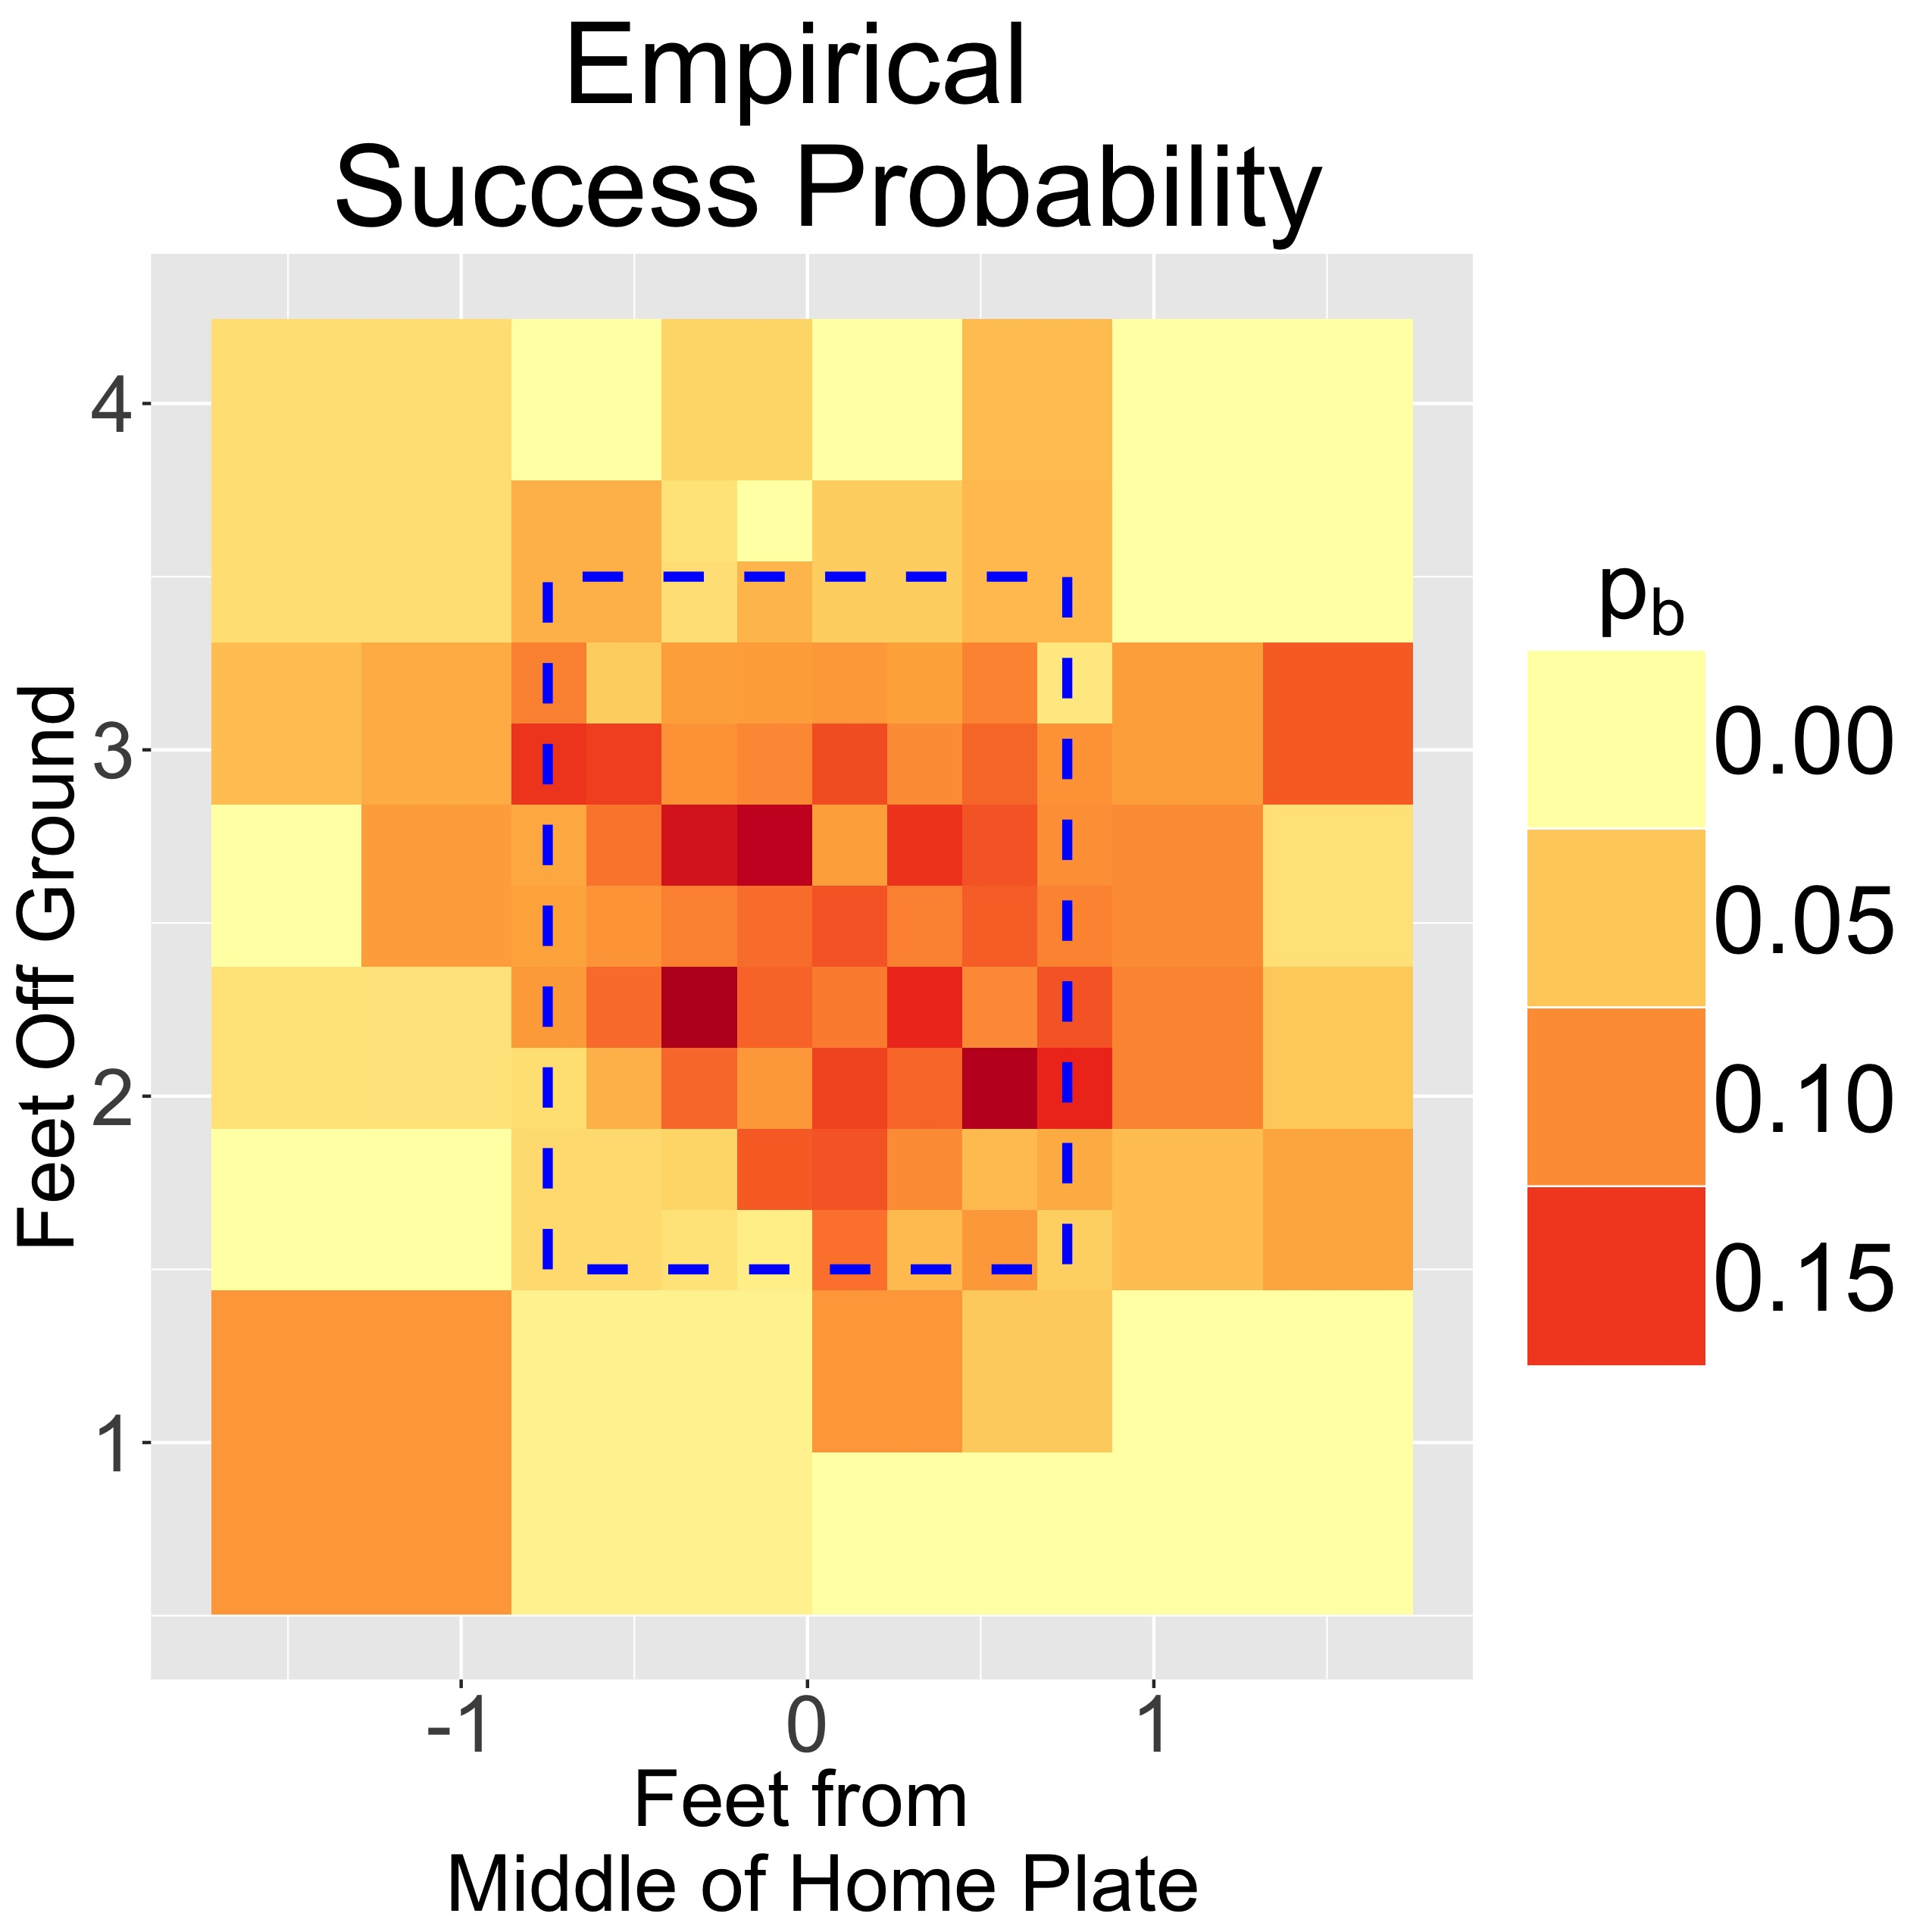
\includegraphics[scale=.04]{Images/Peralta_var-res2.jpg}
	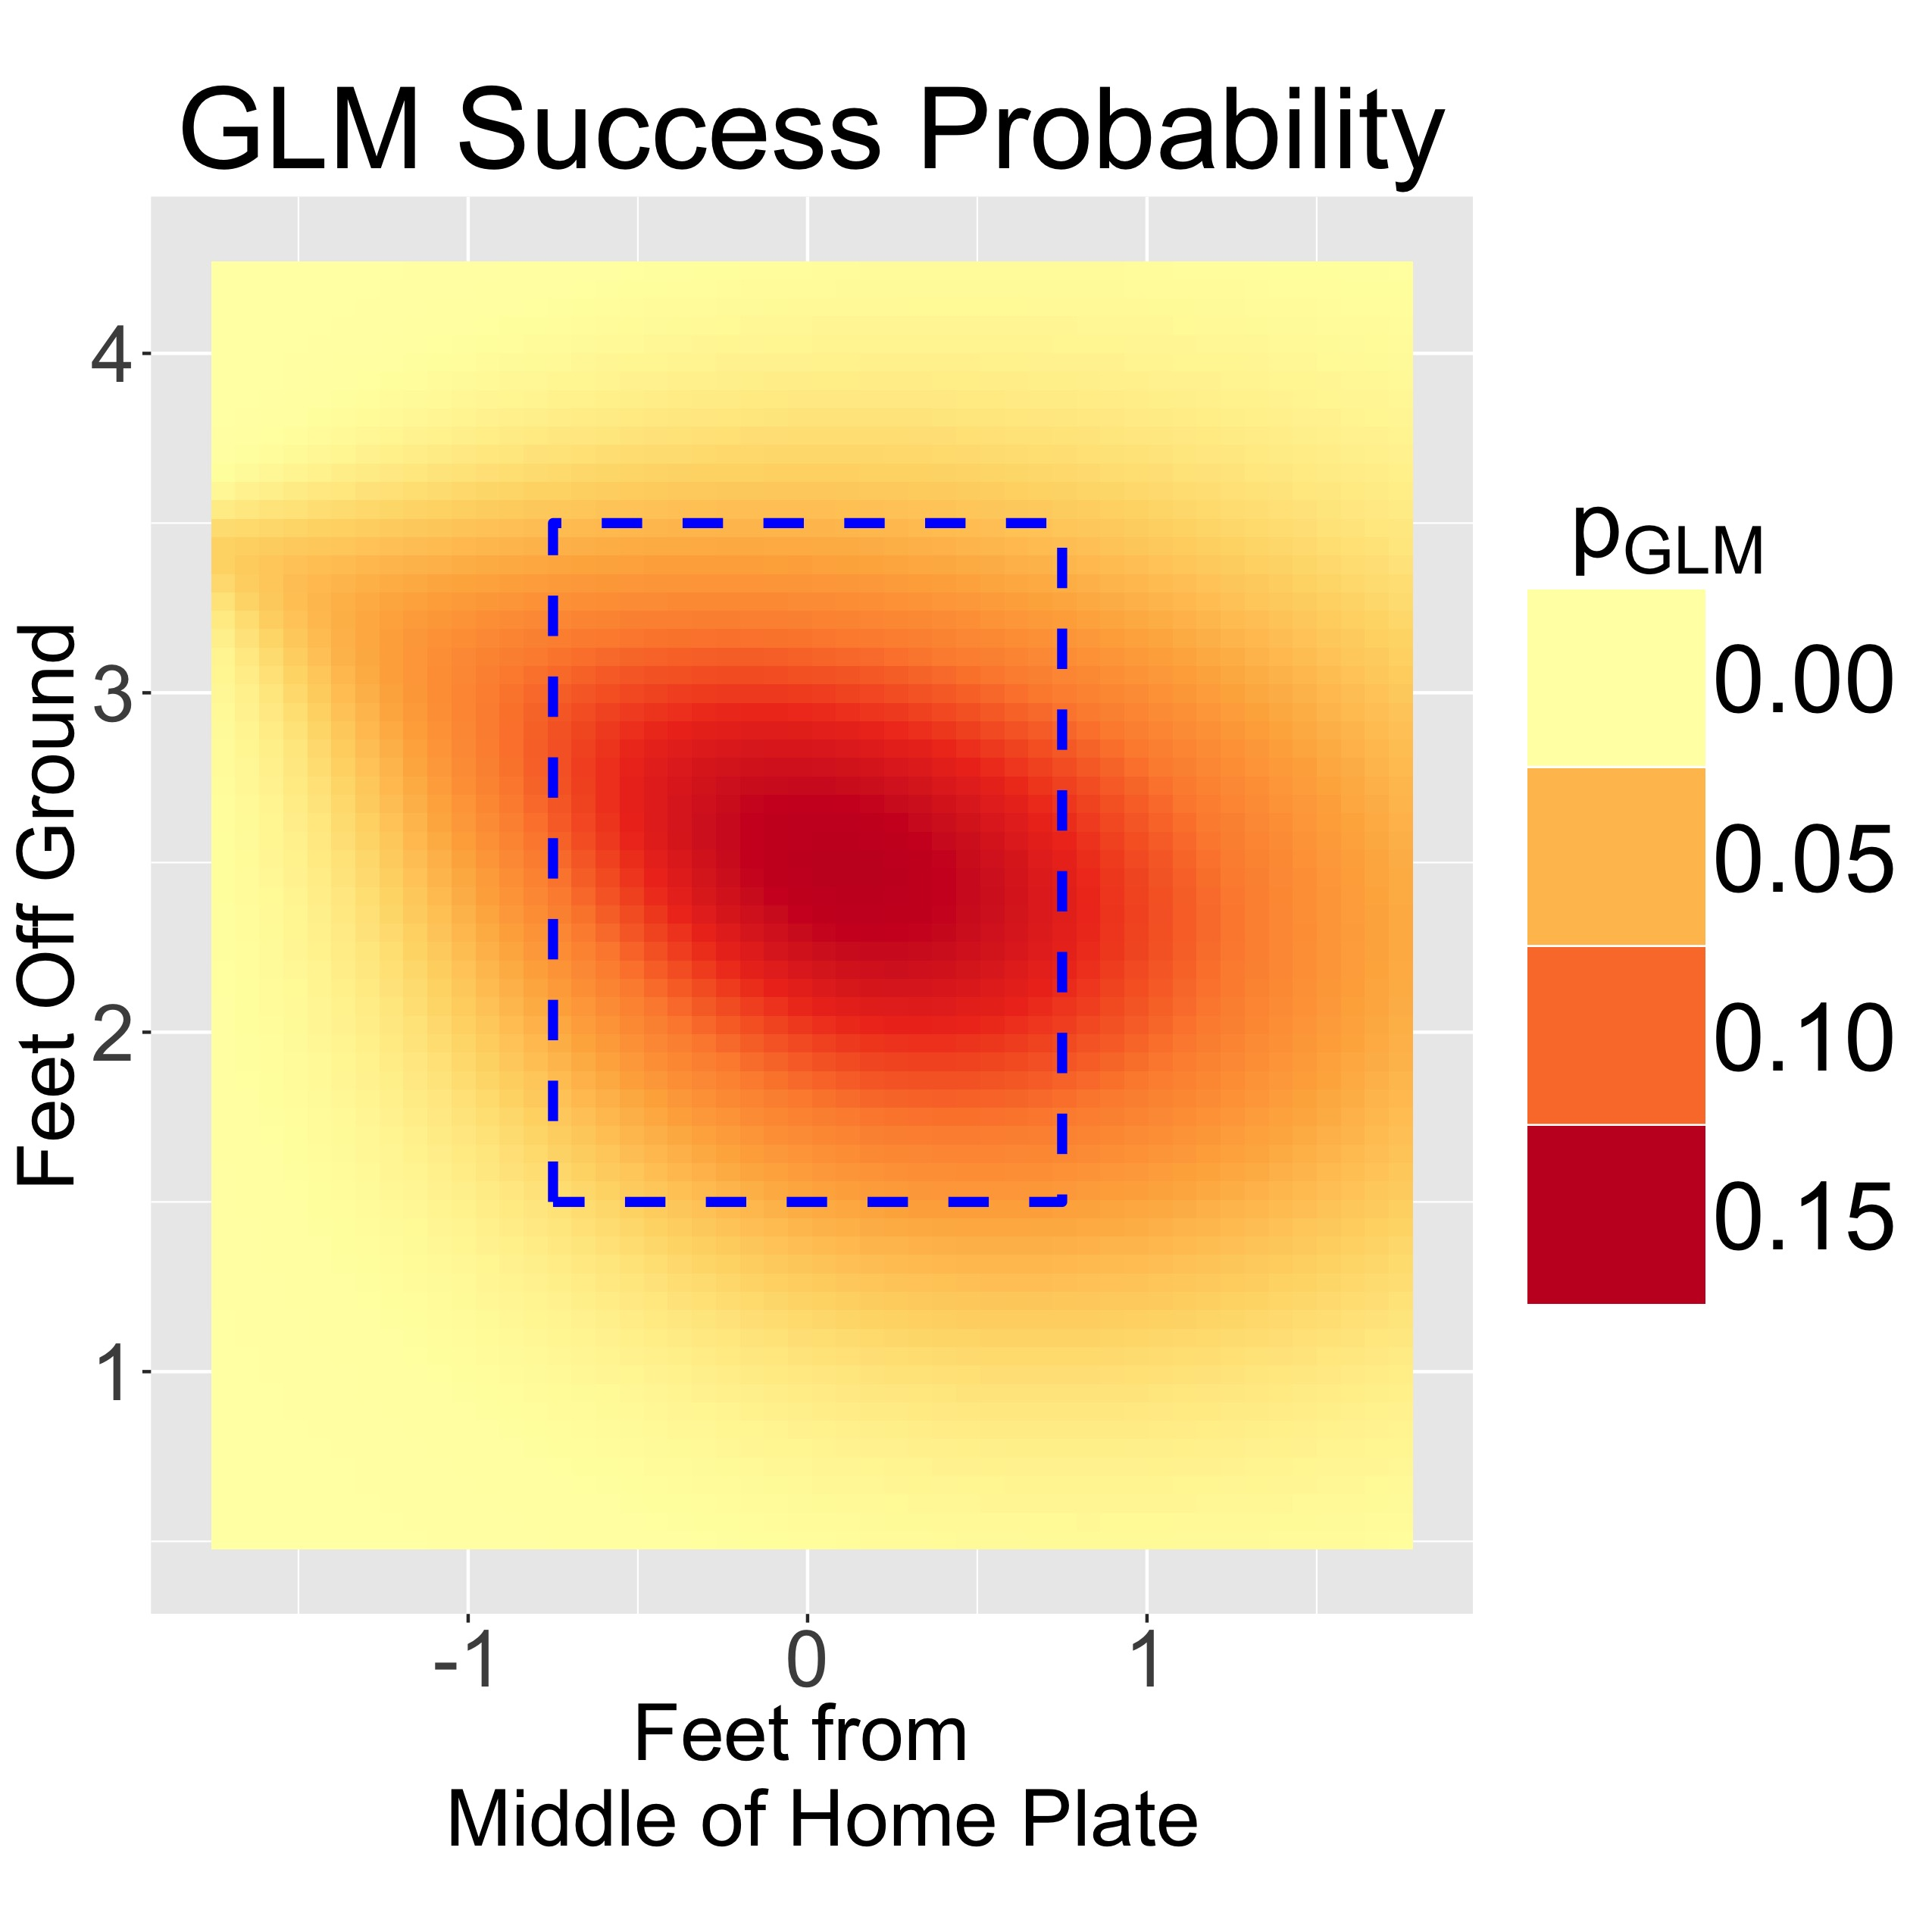
\includegraphics[scale=.04]{Images/Peralta_fit.jpg}
	\end{figure}
\begin{itemize}
\addtolength{\itemsep}{0.5\baselineskip}
\item Hosmer-Lemeshow (logistic regression) GOF test
  \begin{itemize}
  \addtolength{\itemsep}{0.5\baselineskip}
  \item $H_0$: Well fit \\ $H_A$: Lack of fit
  \item p-value = 0.8217
  \end{itemize}
\item Confidence intervals
\end{itemize}
\end{frame}

\begin{frame}{Interactive Confidence Intervals}{} % ======
  \begin{figure}[H]
	\centering
	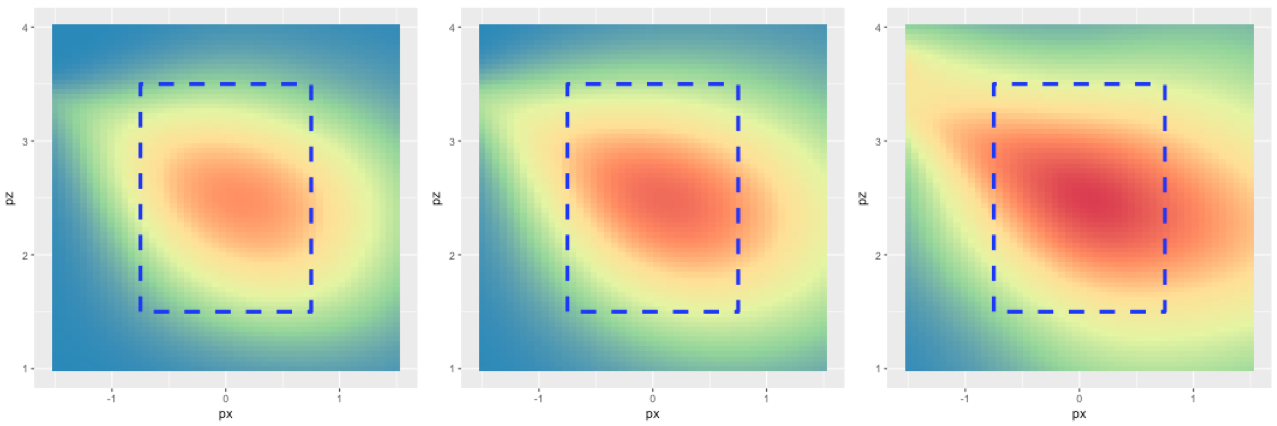
\includegraphics[scale=.275]{Images/99.png}
	\end{figure}
{\bf mapapp}: An R Package
\end{frame}

\begin{frame}[fragile]{{\bf mapapp}: An R Package}
\begin{itemize}
\addtolength{\itemsep}{0.5\baselineskip}
\item Challenge: Where does user stop and package begin?
\item Future improvement
\end{itemize}

\begin{verbatim}
all_in_one <- get_CI(model, x, y, levels)
shinyHMCI(all_in_one)
\end{verbatim}

\begin{enumerate}
\addtolength{\itemsep}{0.5\baselineskip}
\item \verb|get_CI(...)| --- creates proper data structure 
\item \verb|shinyHMCI(all_in_one)| --- creates Shiny app
\end{enumerate}

\end{frame}

\section{Approaches to Big Data Spatial Mixed Models for Baseball Data}

\begin{frame}{Spatial Generalized Linear Mixed Model (SGLMM)}{}
$$ Y_{i}|\mathbf{X}_{i}(\mathbf{s}_{i}) \stackrel{ind}{\sim} \mbox{Bernoulli}(\pi_{i}) $$
$$\text{logit}(\pi_{i}|\pmb{s}_{i}) = \mathbf{X}_{i}(\mathbf{s}_{i})\pmb{\beta} + w(\pmb{s}_{i}) $$
\begin{itemize}
\addtolength{\itemsep}{0.5\baselineskip}
\item $w(\pmb{s}_{i})$ --- spatial random effect, location $\pmb{s}_{i}$.
\item $\pmb{w}(\pmb{s}) = (w(\pmb{s}_{1}), w(\pmb{s}_{2}), \dots, w(\pmb{s}_{N}))$ --- vector
\item $\pmb{w}(\pmb{s})$ - Gaussian Random Field (GRF)
\end{itemize}

\end{frame}

\begin{frame}{Gaussian Random Field: \pmb{w}(\pmb{s})}{} % ======

$$\pmb{w}(\pmb{s}) | \pmb{\theta} \sim \text{MVN}(\pmb{0}, \Sigma(\pmb{\theta}))$$
$$\Sigma(\phi, \sigma^{2})_{i,k} = \sigma^{2} \text{exp}(-||\pmb{s}_{i} - \pmb{s}_{k}||/\phi)$$
\begin{itemize}
\addtolength{\itemsep}{0.5\baselineskip}
\item Spatial exponential covariance
  \begin{itemize}
  \addtolength{\itemsep}{0.5\baselineskip}
  \item $||\pmb{s}_{i} - \pmb{s}_{k}||$ - Euclidean distance
  \item $\sigma^{2}$ - scale parameter
  \item $\phi$ - range parameter.
  \end{itemize}
\item Notice: $\Sigma(\pmb{\theta})$ --- $n \times n$
\end{itemize}

\end{frame}


\begin{frame}{Computational Cost: ``Big N'' Problem}{}
\begin{itemize}
\addtolength{\itemsep}{0.5\baselineskip}
\item Peralta: $n = 9177$
\item $\pmb{w}(\pmb{s})$: $9177 \times 9177$ cov. matrix
\item MCMC iterations require: $\Sigma^{-1}$, determinant of $\Sigma$
\item $\mathcal{O}(n^{3})$ rate of increase: 
$$t(n) \leq M \cdot n^{3}$$ 
$$ \text{as } n \rightarrow \infty$$
\end{itemize}
\end{frame}

\subsection{Computational Optimization in Stan}

\begin{frame}{Hamiltonian Monte Carlo (HMC)}
\begin{itemize}
\addtolength{\itemsep}{0.5\baselineskip}
\item Stan uses Hamiltonian proposal mechanism
\item {\bf Short version}: disk on surface, randomly sample momentum (auxiliary), calculate new position (parameters) --- that's your Metropolis proposal.
        \begin{figure}[H]
      	\centering
      	\includegraphics[scale=.18]{Images/HMC.jpg}
      	\end{figure}
\end{itemize}
\end{frame}


\begin{frame}[fragile]{Stan Computational Optimization}{}
  \begin{itemize}
  \addtolength{\itemsep}{0.5\baselineskip}
  \item  $\phi$, $\pmb{\beta}$: informative/proper priors $\rightarrow$ identifiability/cost/convergence
  \item QR factorization of X, Cholesky decomposition of $\Sigma(\pmb{\theta})$
  \item Matrices \& vectors faster than loops \& scalars
  \item n = 25: 40 seconds $\rightarrow$ 3 seconds
  \item n = 2000 --- overnight, 350 draws
  \end{itemize}
        \begin{figure}[H]
      	\centering
      	\includegraphics[scale=.3]{Images/Turtle.jpg}
      	\end{figure}
\end{frame}

\subsection{Predictive Process Models}

\begin{frame}{Predictive Process Models (PPMs)}{\citep{Banerjee2008}}
\begin{columns}

\column{0.5\textwidth}

\begin{itemize}
\item Knots: $\pmb{S}^{*} = \{\pmb{s}_{1}^{*}, \dots, \pmb{s}_{m}^{*}\}$
      \begin{itemize}
      \item $m < < n$
      \end{itemize}
\end{itemize}

  \begin{figure}[H]
	\centering
	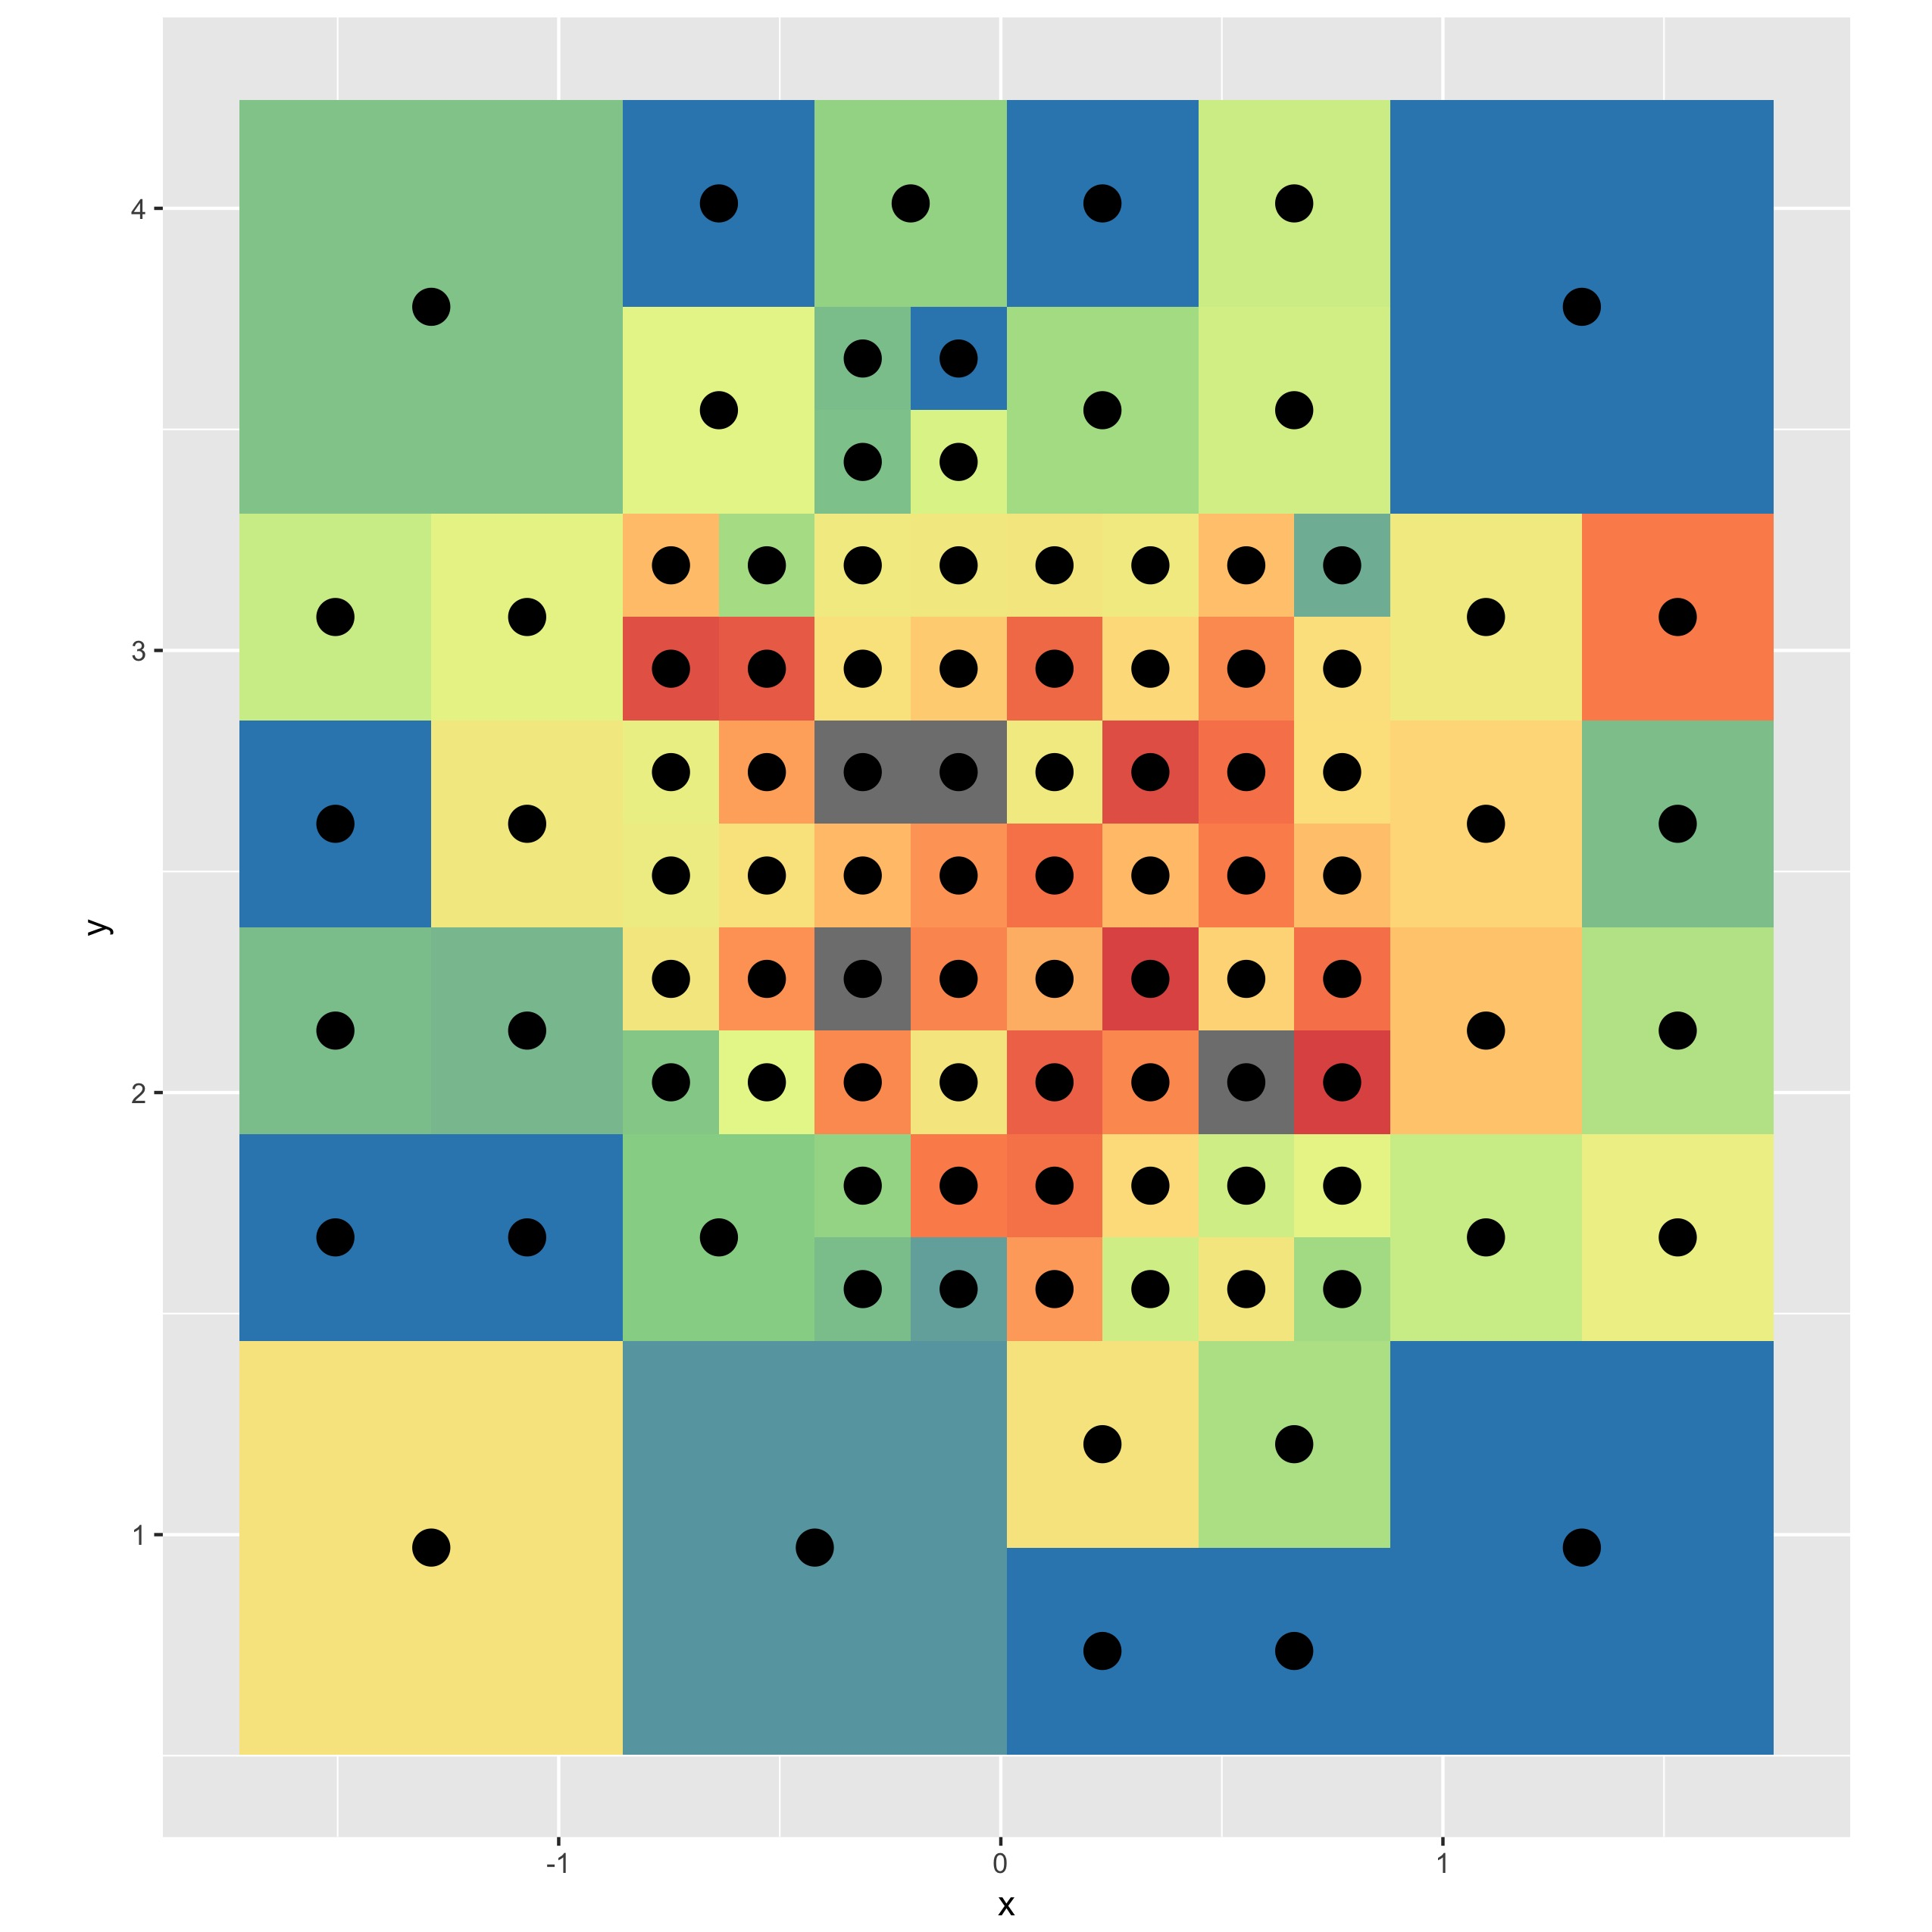
\includegraphics[scale=.045]{Images/knots.jpg}
	\end{figure}

\column{0.5\textwidth}

$$\text{logit}(\pi_{i}|\pmb{s}_{i}) = \pmb{X}_{i}(\pmb{s}_{i}) \pmb{\beta} + \widetilde{w}(\pmb{s}_{i}) $$
$$\widetilde{\pmb{w}}(\pmb{s}) \sim \text{MVN}\{0, \widetilde{\Sigma}(\pmb{\theta})\} $$
$$\widetilde{\Sigma}(\pmb{\theta})_{i,j} = \pmb{\sigma}^{*T}(\pmb{s}_{i};\pmb{\theta}) \cdot \pmb{\Sigma}^{*-1}(\pmb{\theta}) \cdot \pmb{\sigma}^{*}(\pmb{s}_{j};\pmb{\theta})$$
    \begin{itemize}
    \addtolength{\itemsep}{0.5\baselineskip}
    \item $\pmb{\sigma}^{*}(\pmb{s}_{i};\pmb{\theta})$ = $\text{Cov}(\pmb{s}_{i}, \pmb{S}^{*})$
    \item $\pmb{\Sigma}^{*}(\pmb{\theta}) = \text{Var}(\pmb{S}^{*})$
    \end{itemize}

\end{columns}
\end{frame}

\begin{frame}{PPM Results}

\begin{itemize}
\addtolength{\itemsep}{0.5\baselineskip}
\item Implement in {\bf spBayes} \citep{Finley2013}.
\item MCMC chains \textcolor{red}{did not converge}. \\
      \begin{itemize}
      \addtolength{\itemsep}{0.5\baselineskip}
      \item n = 1000, knots = 97, 10K samples, $\approx$ 6.7 mins
      \item n = 1000, knots = 49, 30K samples, $\approx$ 7 mins
      \item n = 3000, knots = 49, 80K samples, $\approx$ 54 mins
      \end{itemize}
\item Speed issue for extending MCMC chains
\item Buzz Lightyear is fast.
\end{itemize}
  \begin{figure}[H]
	\centering
	\includegraphics[scale=.02]{Images/BL.jpg}
	\end{figure}
\end{frame}

\subsection{Integrated Nested Laplace Approximation}

\begin{frame}{INLA Overview}
$$ \text{logit}(\pi_{i}) = \pmb{X}_{i}(\pmb{s}_{i})\pmb{\beta} + w(\pmb{s}_{i}) $$
$$\pmb{w}(\pmb{s}) | \pmb{\theta} \sim \text{MVN}(\pmb{0}, \textcolor{blue}{\Sigma(\pmb{\theta})})$$
\begin{itemize}
\addtolength{\itemsep}{0.5\baselineskip}
\item Bayesian hierarchical models w/ latent GRF
\item Assume \textcolor{blue}{Mat\'ern} covariance
\item Two parts (continuous domain) \\
  \begin{itemize}
  \addtolength{\itemsep}{0.5\baselineskip}
  \item Part 1: Represent GRF as GMRF (SPDE)
  \item Part 2: Integrated Nested Laplace Approximation (INLA)
  \end{itemize}
\end{itemize}
  \begin{figure}[H]
	\centering
	\includegraphics[scale=.0175]{Images/BL.jpg}
	\end{figure}
	
\end{frame}

\begin{frame}{Integrated Nested Laplace Approximation}{\citep{Rue2009}}
  \begin{itemize}
  \addtolength{\itemsep}{0.5\baselineskip}
  \item Parameter vector: $\pmb{\rho} = ( \pmb{\beta}^{\text{T}}, \widetilde{\pmb{w}}^{\text{T}} )^{\text{T}}$
              \begin{itemize}
              \addtolength{\itemsep}{0.5\baselineskip}
              \item $\pmb{Q}$: precision matrix of $\pmb{\rho}$
              \end{itemize}
  \item Hyperparameter vector: $\pmb{\theta} = (\kappa, \sigma )$
  \end{itemize}

\begin{enumerate}
\item Gaussian approximation:

    \begin{align}
    p(\pmb{\rho} |\pmb{\theta},\pmb{y}) & \propto p(\pmb{y}|\pmb{\rho}, \pmb{\theta}) p(\pmb{\rho}|\pmb{\theta}) p(\pmb{\theta}) \nonumber \\
    p(\pmb{\rho}|\pmb{\theta},\pmb{y}) & \propto \text{exp}\left(-\frac{1}{2}\pmb{\rho}^{T}\pmb{Q \rho} + \sum_{i} \text{log }p(y_{i}|\pmb{\rho},\pmb{\theta}) \right) \nonumber \\
    \textcolor{red}{p_{G}(\pmb{\rho}|\pmb{\theta}, \pmb{y})} & \propto \text{exp} \left( -\frac{1}{2}(\pmb{\rho-\mu})^{T} (\pmb{Q} + \text{diag}(\pmb{c}) ) (\pmb{\rho - \mu}) \right) \nonumber
    \end{align}

    \begin{itemize}
    \item $\pmb{c}$ and $\pmb{\mu}$ depend on second order Taylor expansions of $f(\pmb{\rho}) = \sum_{i} \text{log }p(y_{i}|\pmb{\rho},\pmb{\theta})$
    \end{itemize}

\end{enumerate}
\end{frame}


\begin{frame}{Integrated Nested Laplace Approximation} {\citep{Rue2009}}
\begin{itemize}
\item Fact: $P(A,B) = P(A|B) P(B) = P(B|A) P(A)$
$$ p(\pmb{y} | \pmb{\theta}) = \frac{p(\pmb{y} | \pmb{\rho}, \pmb{\theta}) p(\pmb{\rho} | \pmb{\theta})} {p(\pmb{\rho} | \pmb{y}, \pmb{\theta})} $$
\item Bayes proportionality:
    \begin{align}
    p(\pmb{\theta}|\pmb{y}) & \propto p(\pmb{y}|\pmb{\theta})p(\pmb{\theta}) \nonumber \\
    & \propto \frac{p(\pmb{y} | \pmb{\rho}, \pmb{\theta}) p(\pmb{\rho} | \pmb{\theta})}{p(\pmb{\rho} | \pmb{y}, \pmb{\theta})} \cdot p(\pmb{\theta}) \nonumber
    \end{align}
\end{itemize}

\begin{enumerate}
\setcounter{enumi}{1}
\item For a given $\pmb{\theta}$, let $\pmb{\rho}_{0} = \text{argmax}_{\rho}p(\pmb{\rho}|\pmb{y},\pmb{\theta})$. Then,

$$ \textcolor{blue}{\tilde{p}(\pmb{\theta}|\pmb{y})}  \propto  \frac{p(\pmb{y} | \pmb{\rho}_{0}, \pmb{\theta}) p(\pmb{\rho}_{0} | \pmb{\theta})}{p_{G}(\pmb{\rho}_{0} | \pmb{y}, \pmb{\theta})} \cdot p(\pmb{\theta}) $$

% $ \rightarrow \hat{\pmb{\theta}}_{\text{ML}} \approx \text{argmax}_{\pmb{\theta}} \tilde{p}(\pmb{\theta}|\pmb{y})$

\end{enumerate}
\end{frame}

\begin{frame}{Integrated Nested Laplace Approximation} {\citep{Rue2009}}
\begin{enumerate}
\setcounter{enumi}{2}
\item Numerical integration:
        $$ p(\rho_{j} | \pmb{y}) \approx \int \textcolor{red}{p_{\text{G}}(\rho_{j}|\pmb{\theta, y})} \textcolor{blue}{\tilde{p}(\pmb{\theta}|\pmb{y})} d\pmb{\theta} $$
\item Numerical integration:
$$ p(\theta_{k} | \pmb{y}) \approx \int \textcolor{blue}{\tilde{p}(\pmb{\theta}|\pmb{y})} d\pmb{\theta}_{-k} $$
\end{enumerate}
\end{frame}


\begin{frame}{INLA Model Fit: 34 seconds}{}
\begin{center}
\huge{34 seconds!}
\end{center}
  \begin{figure}[H]
	\centering
	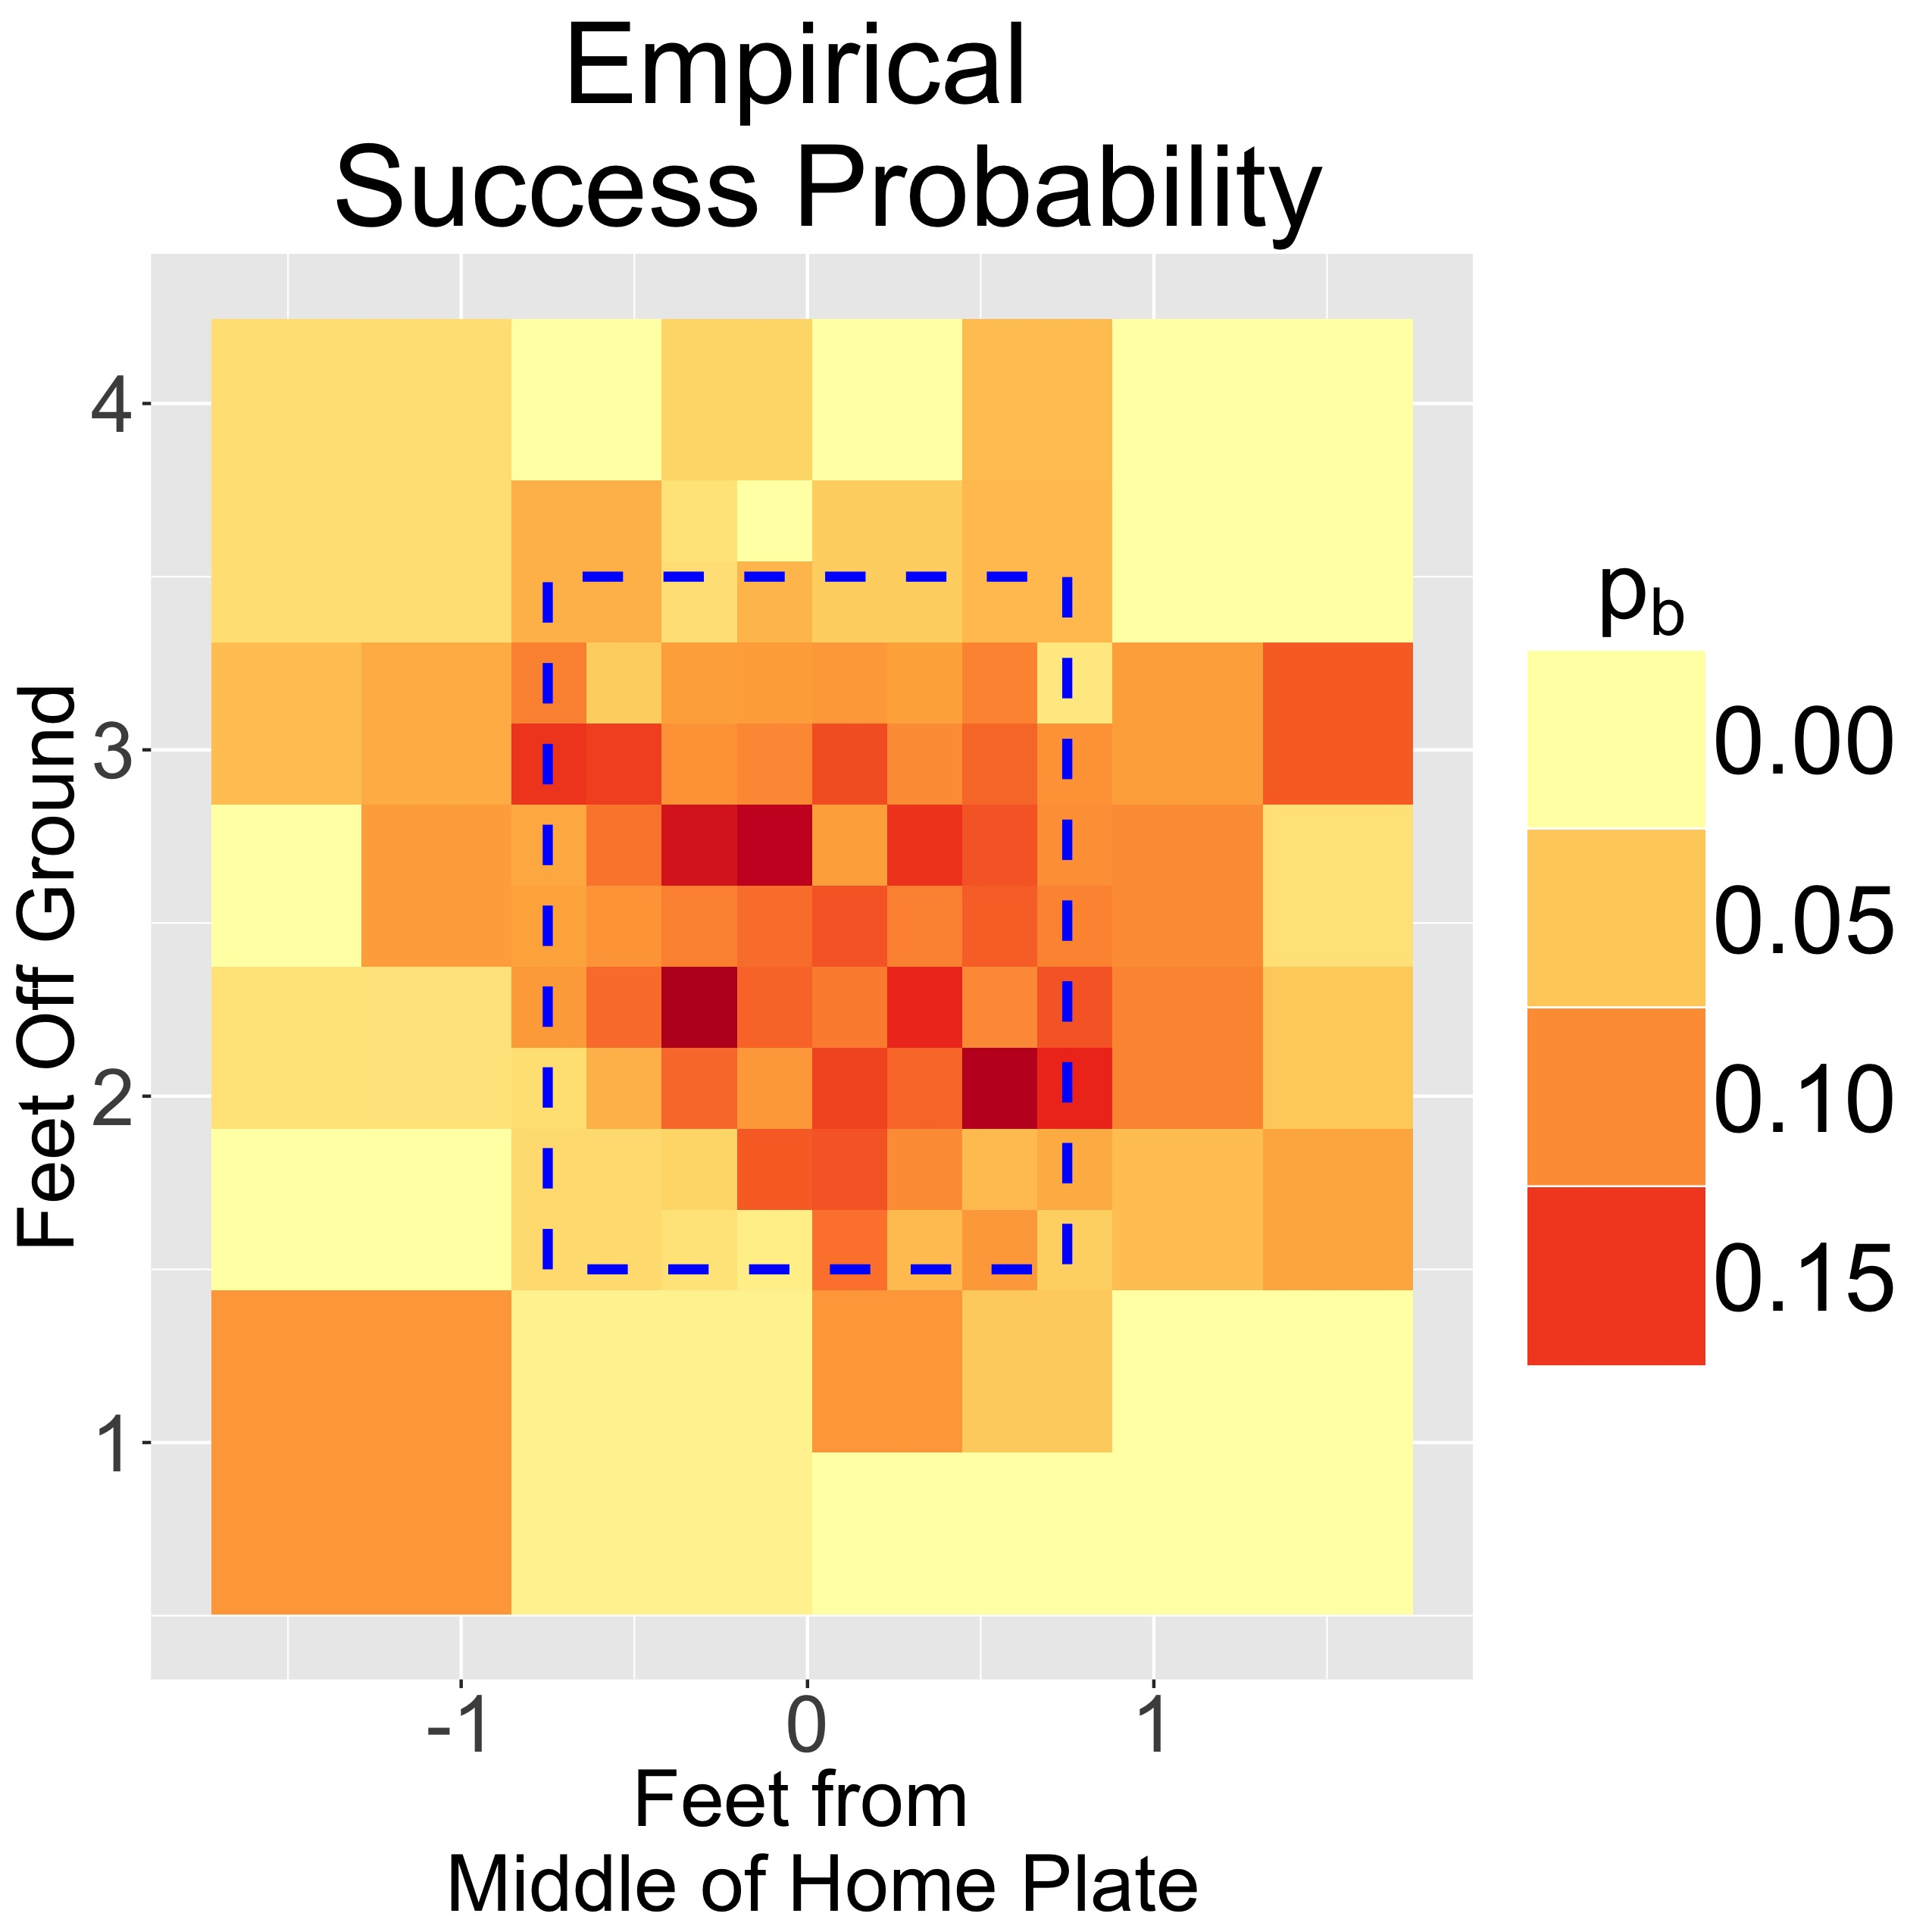
\includegraphics[scale=.045]{Images/Peralta_var-res2.jpg}
	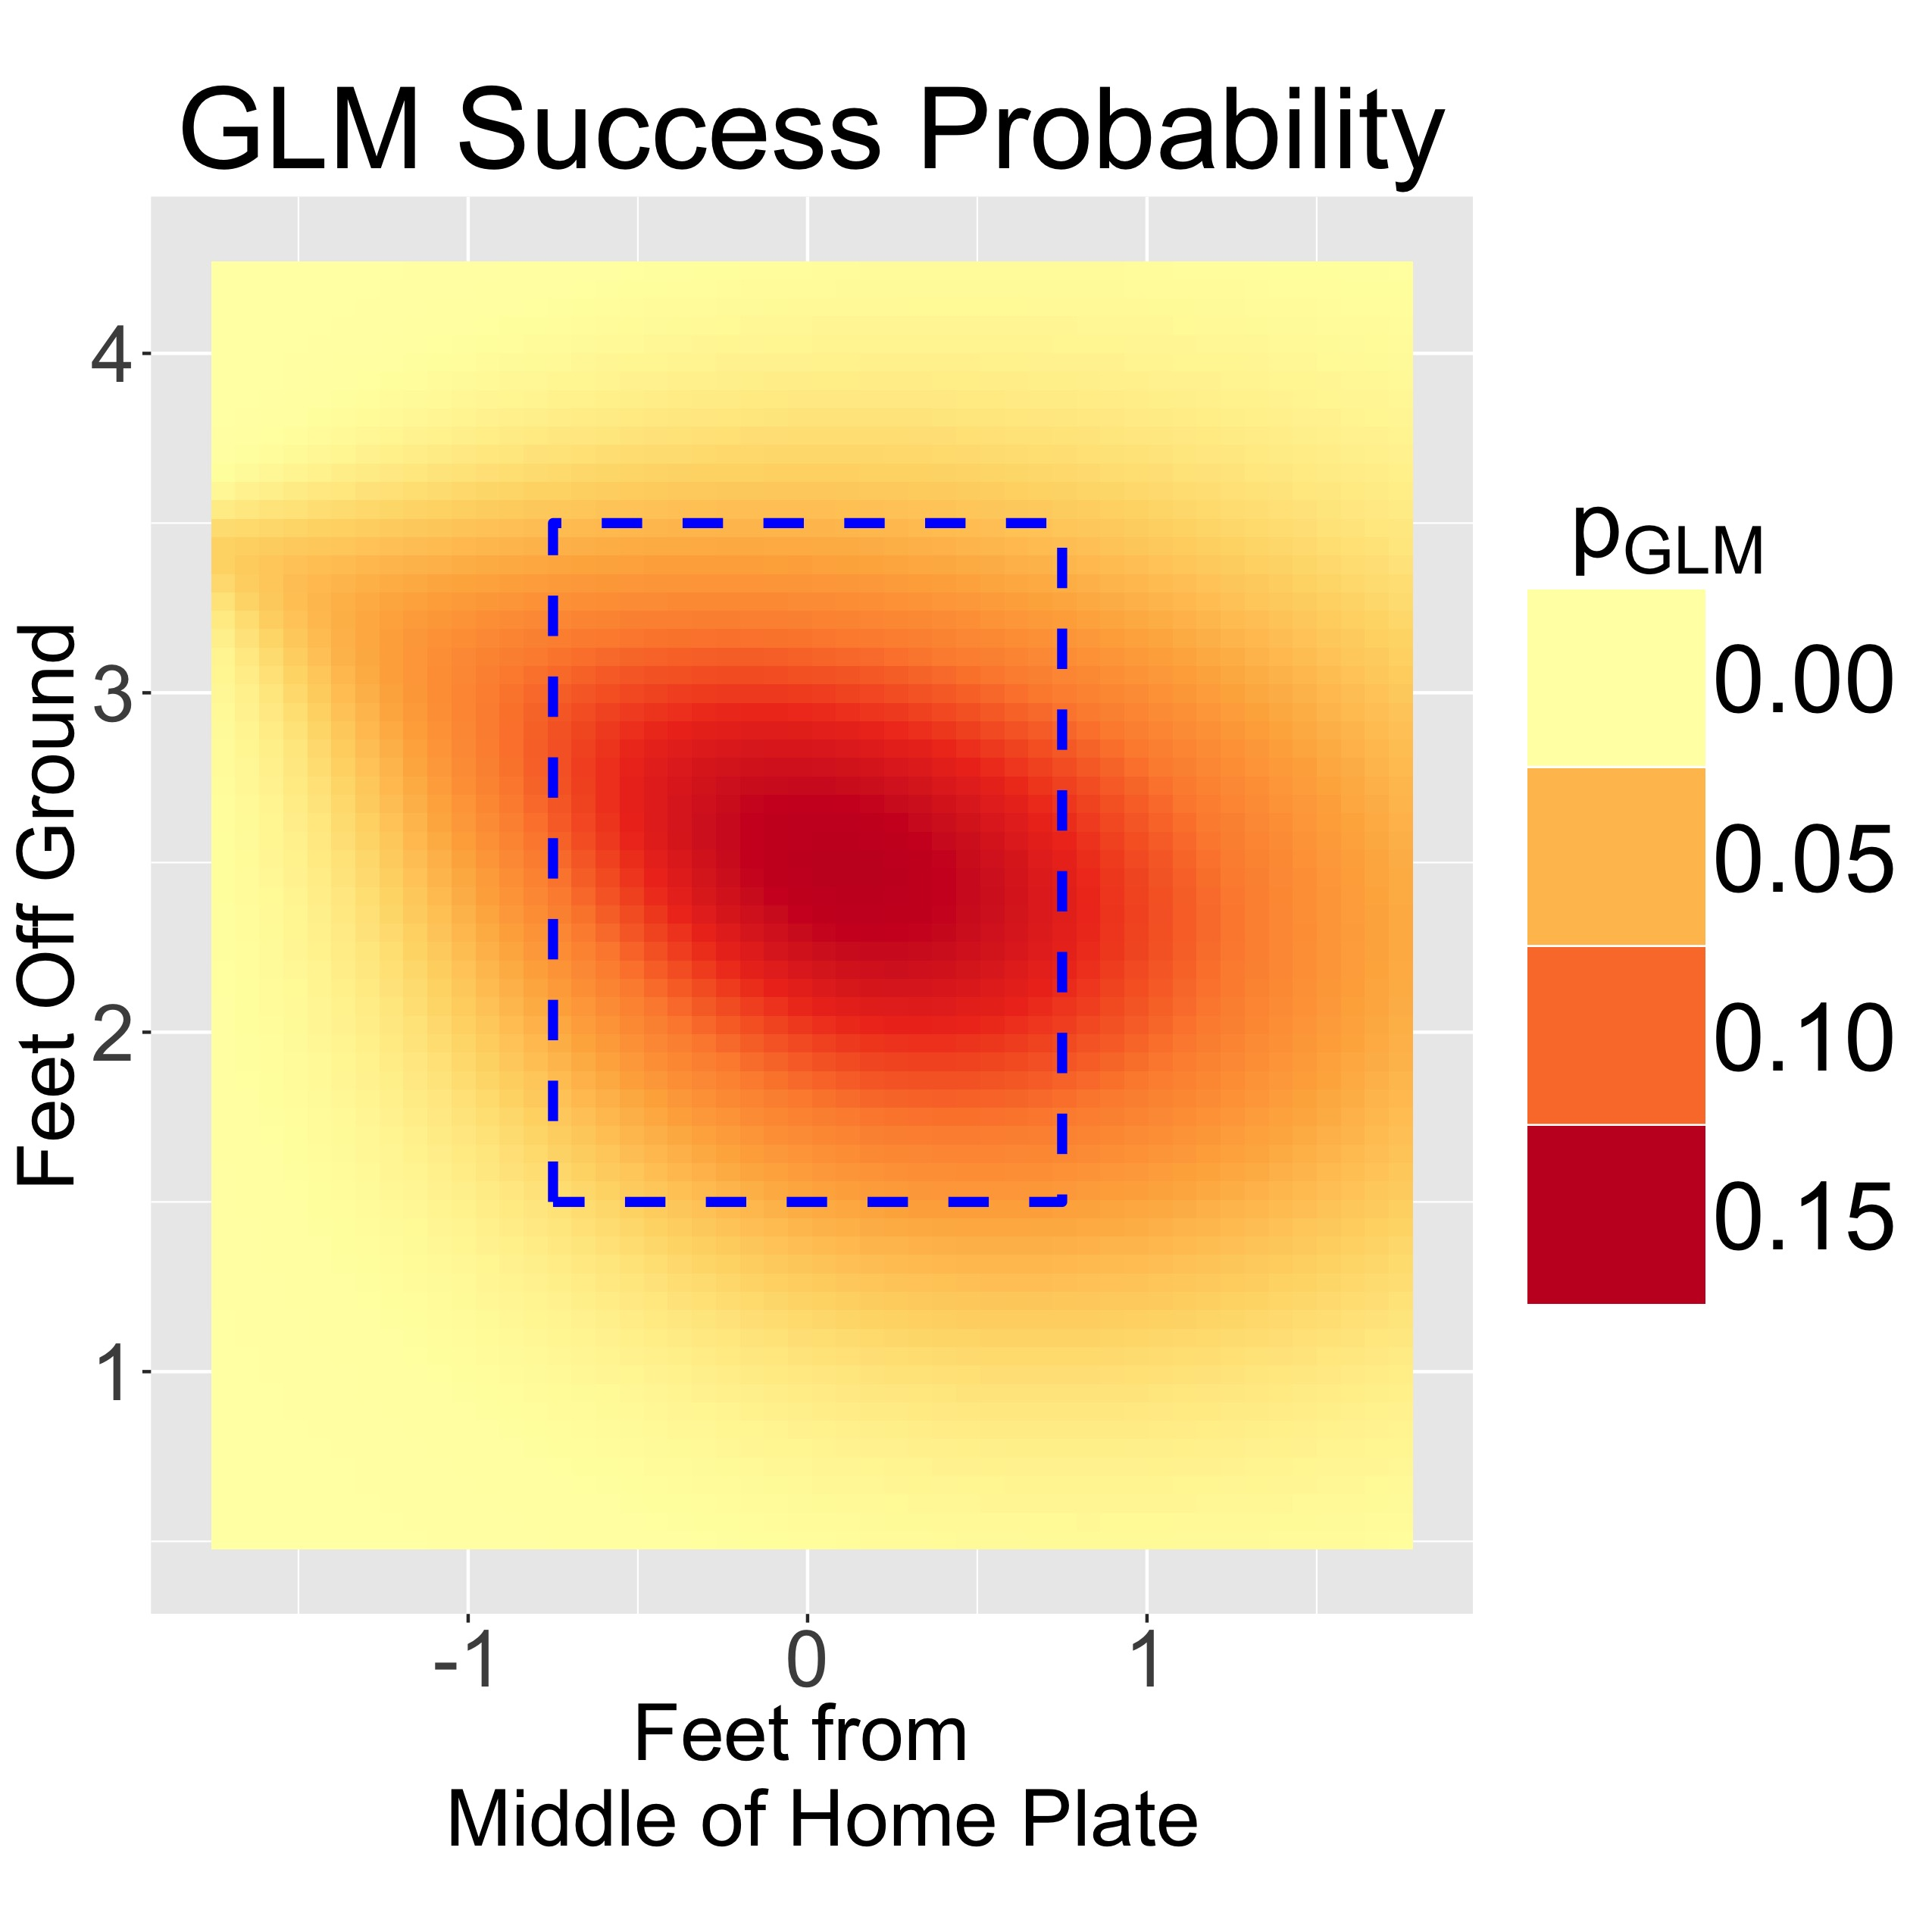
\includegraphics[scale=.045]{Images/Peralta_fit.jpg}
	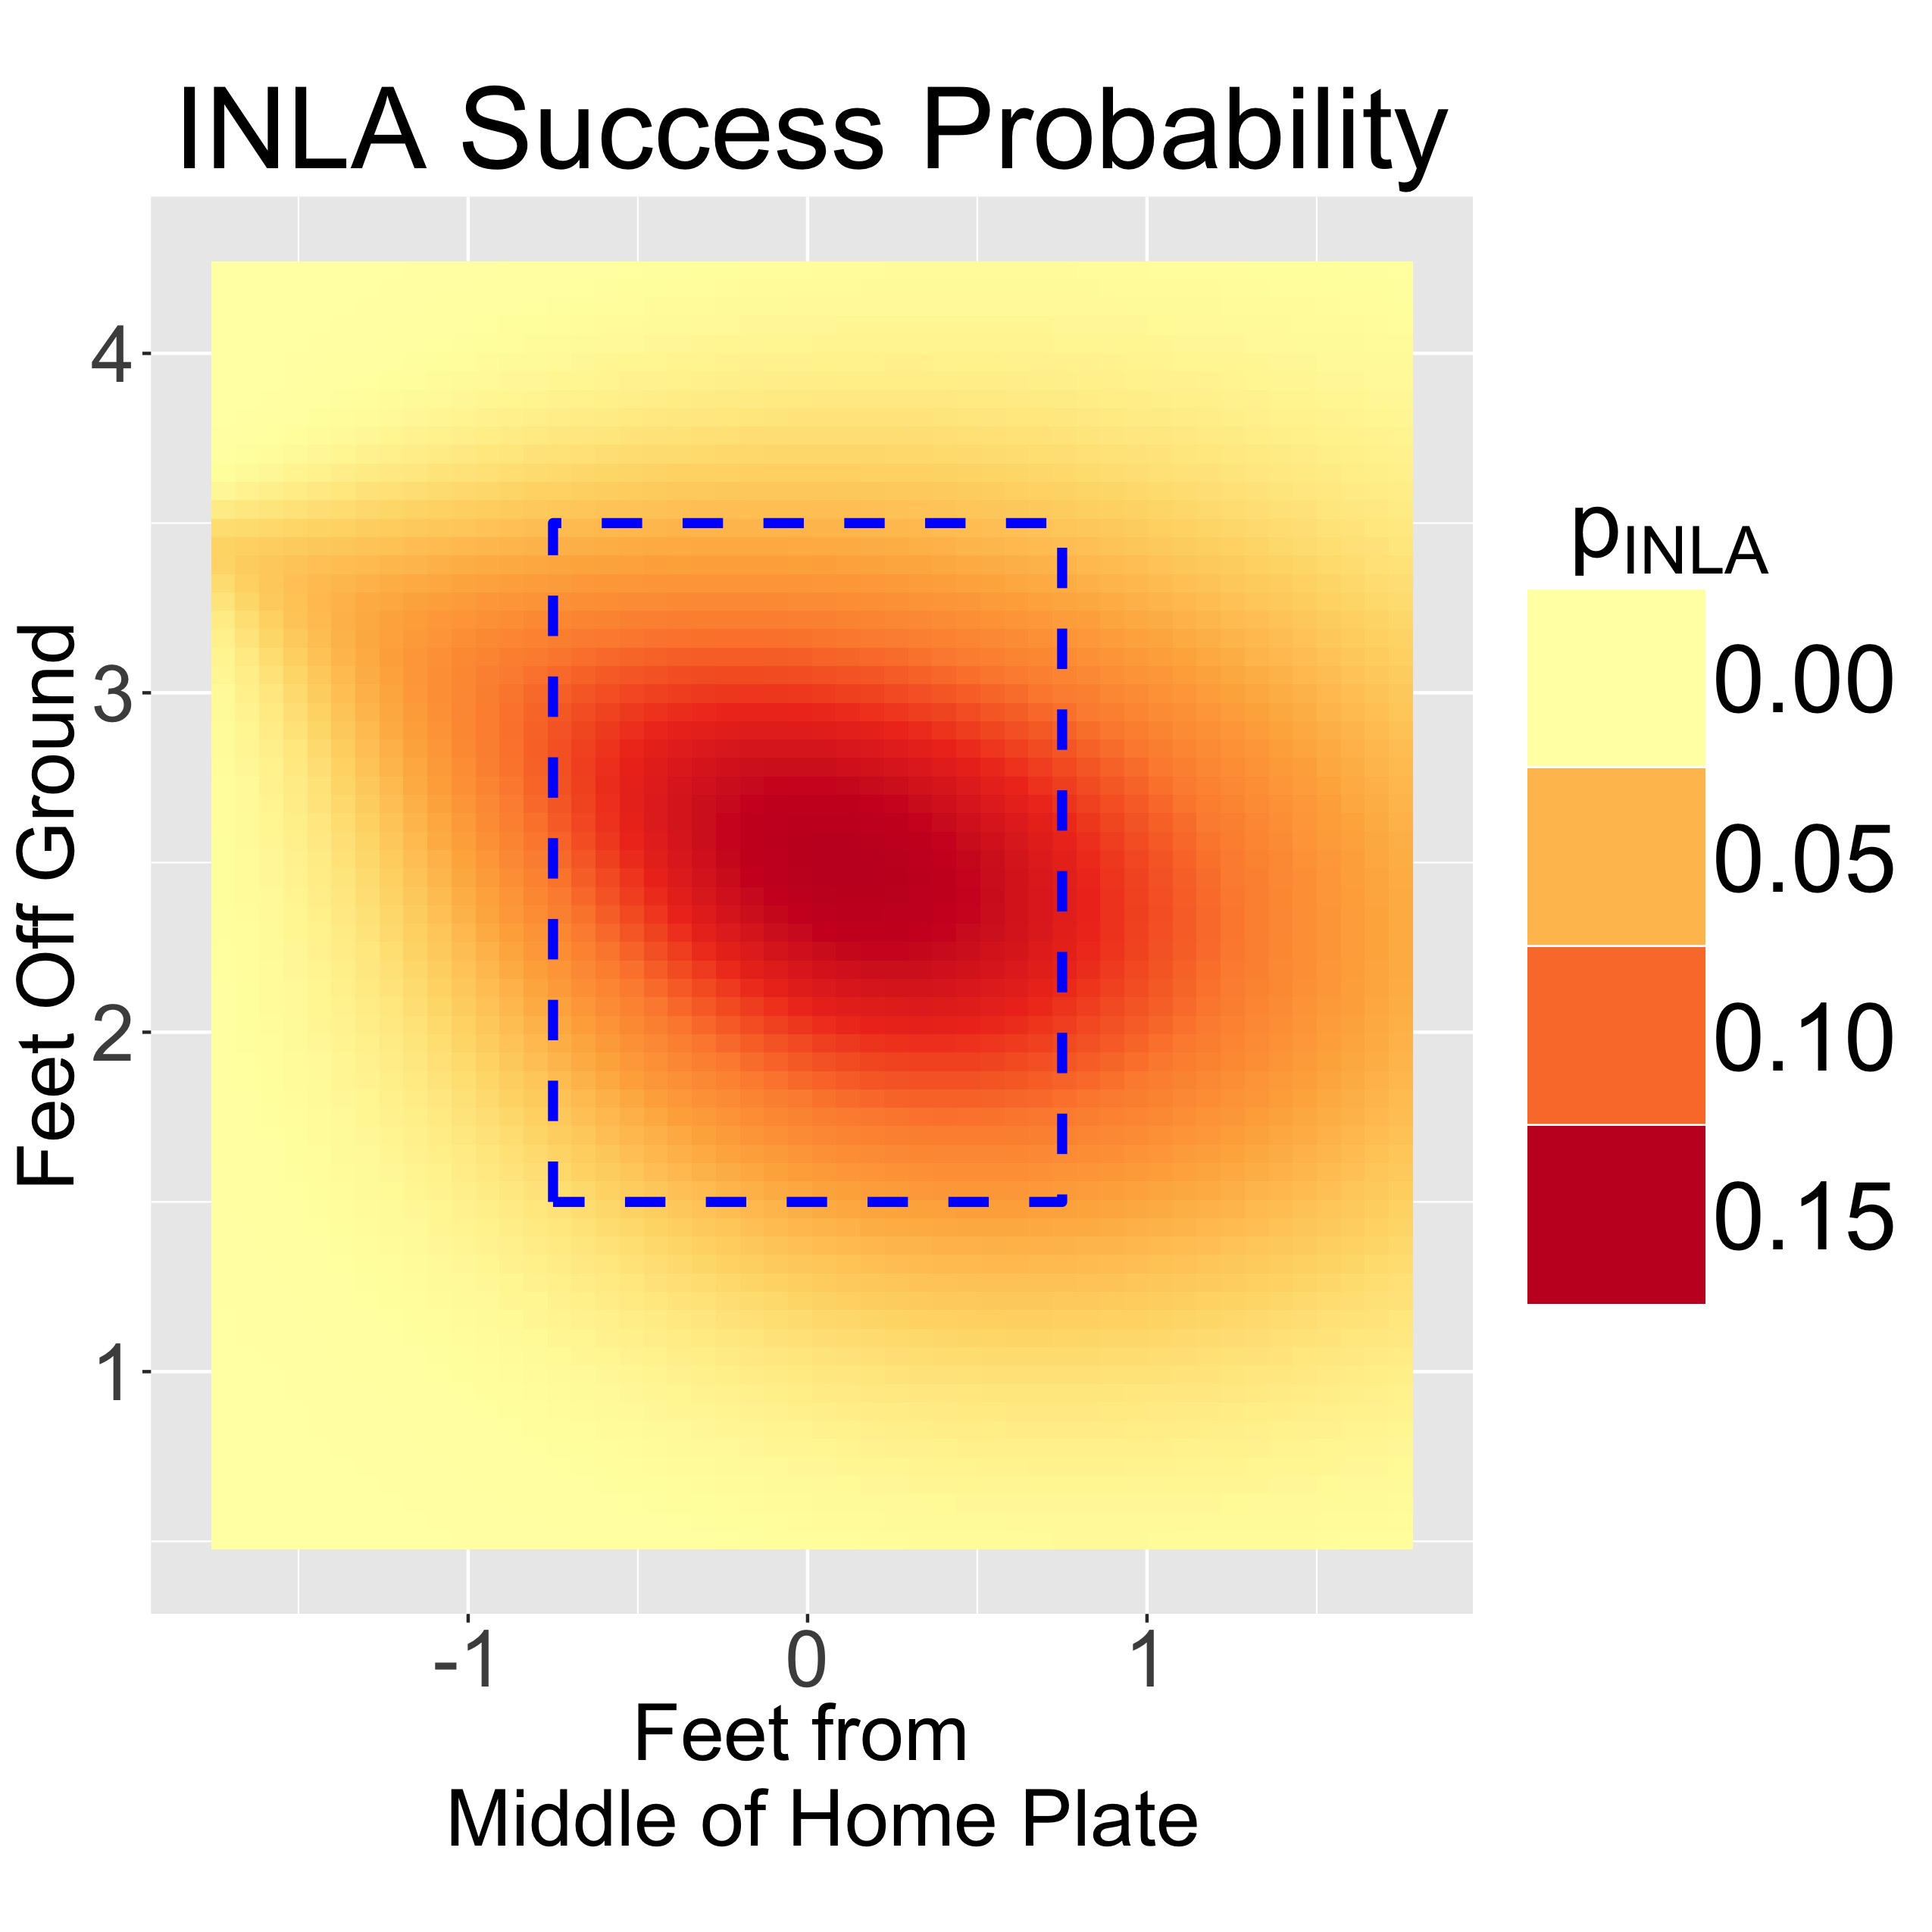
\includegraphics[scale=.045]{Images/INLA.jpg}
	\end{figure}
\end{frame}

\begin{frame}{Estimates}

\begin{table}
\scalebox{0.85}{
\begin{tabular}{| l | c | c | c |}
\hline
\multicolumn{4}{|c|}{} \\
\multicolumn{4}{|c|}{} \\
\multicolumn{4}{|c|}{GLM} \\
\hline
Covariate         & $\beta_{i}$ & MLE   & SE   \\ \hline
1                 & $\beta_{0}$ & -4.08 & 0.70 \\ \hline
r                 & $\beta_{1}$ &  1.19 & 0.51 \\ \hline
$\theta$          & $\beta_{2}$ & -1.93 & 1.90 \\ \hline
$r*\theta$        & $\beta_{3}$ & -1.64 & 0.70 \\ \hline
$r^{2}$           & $\beta_{4}$ & -0.32 & 0.09 \\ \hline
$\theta^{2}$      & $\beta_{5}$ & -3.92 & 1.10 \\ \hline
$r^{2}*\theta^{2}$& $\beta_{6}$ & -0.46 & 0.21 \\ \hline
\end{tabular}
\quad
\begin{tabular}{| l | c | c | c |}
\hline
\multicolumn{4}{|c|}{INLA} \\
\hline
Covariate         & $\rho _{i}$ & $\hat{\rho}_{i}$ & SE \\ \hline
N/A               & $\kappa$    &  3.23 & $\pm$ 1 SE: (1.35, 7.54) \\ \hline
N/A               & $\sigma$    &  0.11 & $\pm$ 1 SE: (0.05, 0.26) \\ \hline
1                 & $\beta_{0}$ & -4.14 & 0.76 \\ \hline
r                 & $\beta_{1}$ &  1.25 & 0.55 \\ \hline
$\theta$          & $\beta_{2}$ & -1.90 & 1.96 \\ \hline
$r*\theta$        & $\beta_{3}$ & -1.70 & 0.93 \\ \hline
$r^{2}$           & $\beta_{4}$ & -0.33 & 0.10 \\ \hline
$\theta^{2}$      & $\beta_{5}$ & -3.93 & 1.14 \\ \hline
$r^{2}*\theta^{2}$& $\beta_{6}$ & -0.48 & 0.22 \\ \hline
\end{tabular}
}
\end{table}
\begin{itemize}
\item $\hat{\kappa}$ --- long range correlation
\item $\text{SE}(w(\pmb{s})) = 0.11$.
\item $\rightarrow 0.15 \pm 1 \cdot \text{SE} = (0.137, 0.165)$
\item $\rightarrow 0.15 \pm 2 \cdot \text{SE} = (0.125, 0.181)$
\end{itemize}
\end{frame}

\begin{frame}{Summary}
\begin{itemize}
\addtolength{\itemsep}{0.5\baselineskip}
\item Resolution selection? Variable-resolution heat maps and {\bf varyres}
\item Heat map confidence intervals? Interactive HMCIs and {\bf mapapp}
\item Fitting big data SGLMMs to baseball data?
  \begin{itemize}
  \addtolength{\itemsep}{0.5\baselineskip}
  \item Stan - insufficient
  \item PPM - Slow and did not converge; to be continued...
  \item INLA - Fast, successful; to be continued...
  \end{itemize}
\end{itemize}
\end{frame}

%
% \begin{itemize}
% \addtolength{\itemsep}{0.5\baselineskip}
% \item Computational costs - increase at a rate of $\mathcal{O}(n^{3/2})$
% \item Trade-offs - speed for bias (Binomial data)
% \end{itemize}
%
% \begin{frame}{Next Steps}
% \begin{itemize}
% \addtolength{\itemsep}{0.5\baselineskip}
% \item Model evaluation, scoring rules \citep{Bickel2007}
% \item Cross validation study
% \end{itemize}
% \end{frame}
%
\begin{frame}{}
\begin{center}
\Huge{Thanks for listening.}
\end{center}
\end{frame}

\bibliography{Baseball}

\begin{frame}{Moving Forward}
\begin{itemize}
\addtolength{\itemsep}{0.5\baselineskip}
\item Improve packages
\item Submit packages to CRAN 
\item Biomechanists at OSU
\item Compare GLM and SGLMM with scoring rules
\item Exit velocity as response variable
\item Independence assumption, pitch sequences
\item Randomized pitch selection
\end{itemize}

\end{frame}

% \begin{frame}{If I knew then...}
%   \begin{itemize}
%   \addtolength{\itemsep}{0.5\baselineskip}
%   \item Skip UNC
%   \item Start research $\rightarrow$ start packages 
%   \item Use courses to practice writing, get feedback, etc.
%   \item Emphasize literature review
%   \end{itemize}
% Glad I did know...
%   \begin{itemize}
%   \addtolength{\itemsep}{0.5\baselineskip}
%   \item ``Write and show as you go.''
%   \item Growth mindset
%   \end{itemize}
% 
% \end{frame}
% 
% \begin{frame}{Responsibilities}
%     \begin{itemize}
%     \addtolength{\itemsep}{0.5\baselineskip}
%     \item Reproducibility.
%     \item Acknowledge uncertainty.
%     \item Honesty
%           \begin{itemize}  
%           \addtolength{\itemsep}{0.5\baselineskip}
%           \item Expertise
%           \item Data
%           \item Methods
%           \item Results
%           \end{itemize}
%     \item Warren Buffet anecdote
%     \end{itemize}
% \end{frame}
% 
% \begin{frame}{Important Theorems}
%     \begin{itemize}
%     \addtolength{\itemsep}{0.5\baselineskip}
%     \item Law of Large Numbers - ``Guarantees stable, long term results for random events.''
%     \item Central Limit Theorem
%     \item Bayes Theorem
%     \item Taylor's Theorem
%     \item Ito's Lemma - stochastic calculus, mathematical finance, Black-Scholes, options pricing!
%     \end{itemize}
% \end{frame}
% 
% \begin{frame}[fragile]{Variable-Resolution Algorithm}{Pseudo-code}
% * Keep track of three containers: History, Current, Iteration
% \begin{verbatim}
% function(dataset,
%          fun = mean, # function to apply to box data
%          cutoff,     # stopping rule threshold
%          max ){      # maximum number of iterations
% 
% HISTORY_CONTAINER # store iterative results
% 
% CURRENT_CONTAINER: box centers, statistic,
%   box observations, box heights/widths,
%   box vert/horiz, upper/lower bounds
% 
% Add CURRENT_CONTAINER to HISTORY_CONTAINER
% \end{verbatim}
% \end{frame}
% 
% \begin{frame}[fragile]{Variable-Resolution Algorithm}{Pseudo-code}
% \begin{verbatim}
% WHILE(exists N_b > cutoff and ITERATION < max) {
%   ITERATION CONTAINER <- list()
% 
%     FOR(All BOX_b in CURRENT CONTAINER){
%       IF(BOX_b count > cutoff){
% 
%           Retrieve BOX_b data, subdivide/calculate
%             BOX_b sub-box info, add to
%             ITERATION CONTAINER
%       }
%     }
%     Update CURRENT_CONTAINER: remove obsolete boxes,
%       add ITERATION CONTAINER boxes
%     Add CURRENT CONTAINER to HISTORY CONTAINER
%   }
% 
% \end{verbatim}
% \end{frame}
% 
% 
% \begin{frame}{HMC, Longer Version}
%   \begin{itemize}
%   \addtolength{\itemsep}{0.5\baselineskip}
%   \item $H(q(t),p(t)) = U(\textcolor{blue}{q(t)}) + K(p(t))$
%   \item Total energy of a system
%   \item t = time
%   \item \textcolor{blue}{q = position} (variables of interest), U = potential energy
%   \item p = momentum (auxiliary), K = kinetic energy
%   \item $H(q,p) = -\log \textcolor{blue}{f_{q}(q)} + p^{T}\pmb{M}^{-1}p/2$
%   \item Tidy partial derivatives
%   \end{itemize}
% \end{frame}
% 
% \begin{frame}[fragile]{Stan Optimization}
% \begin{itemize}
% \item QR factorization of X
%     \begin{align*}
%     \pmb{X} &= \pmb{QR} \\
%     \pmb{X \beta} &= \pmb{QR \beta} \rightarrow \text{Let } \pmb{\theta} = \pmb{R \beta} \\
%     \pmb{X \beta} &= \pmb{Q \theta} \\
%     \pmb{\beta} &= \pmb{R^{-1}\theta}
%     \end{align*}
% \item Cholesky decomposition of $\Sigma(\pmb{\theta})$
%     \begin{verbatim}
%     L = cholesky_decompose(Sigma);
%     Z ~ normal(0, 1);
%     Z_mod = L * Z;
%     Y ~ bernoulli_logit(Q*theta + Z_mod);
%     \end{verbatim} 
% \end{itemize}
% \end{frame}
% 
% \begin{frame}{Stan Model Fitting} % ===== ====== ===== ===== =====
% \begin{itemize}
% \addtolength{\itemsep}{0.5\baselineskip}
% \item N = 1000: 7 hours 45 mins for 1500 draws
%       \begin{itemize}
%       \item Note: GLM (w/o spatial effect): 6 seconds.
%       \end{itemize}
% \item N = 2000 overnight, 350 draws
% \end{itemize}
%   \begin{figure}[H]
% 	\centering
% 	\includegraphics[scale=.25]{Images/Turtle.png}
% 	\end{figure}
% \end{frame}
% 
% \begin{frame}{Predictive Process Models (PPMs) }{\citep{Banerjee2008}} % ===== ====== ===== ===== =====
% \begin{itemize}
% \addtolength{\itemsep}{1\baselineskip}
% \item $\text{Cov}\left(w(\pmb{s}_{i}), w(\pmb{s}_{k}) \right) = \Sigma(\pmb{s}_{i}, \pmb{s}_{k}; \pmb{\theta})= \big[\Sigma(\pmb{s}_{i}, \pmb{s}_{k}; \pmb{\theta}) \big]_{i,k=1}^{n}$
% \item Knots: $\pmb{S}^{*} = \{\pmb{s}_{1}^{*}, \dots, \pmb{s}_{m}^{*}\}$
%   \begin{itemize}
%   \item $m < < n$
%   \end{itemize}
% \item Knot random effects: $\pmb{w}^{*} = \left[w(\pmb{s}_{i}^{*})\right]_{i=1}^{m}$
% \item Knot GRF: $\pmb{w}^{*}|\pmb{\theta} \sim \text{MVN}\{\pmb{0}, \Sigma^{*}(\pmb{\theta})\}$ --- $m$-dim \\
%   \begin{itemize}
%   \addtolength{\itemsep}{0.5\baselineskip}
%   \item Knot covariance: $\Sigma^{*}(\pmb{\theta}) = \big[\Sigma(\pmb{s}_{i}^{*}, \pmb{s}_{k}^{*})\big]_{i,k = 1}^{m}$
%   \end{itemize}
% \item $\pmb{\sigma}(\pmb{s}_{0};\pmb{\theta}) = \left[\Sigma(\pmb{s}_{0}, \pmb{s}_{k}^{*}; \pmb{\theta})\right]_{k = 1}^{m}$ --- $m \times 1$ vector
% \end{itemize}
% \end{frame}
% 
% \begin{frame}{PPM Kriging} % ===== ====== ===== ===== =====
% \begin{itemize}
% \addtolength{\itemsep}{0.5\baselineskip}
% \item $\pmb{\sigma}(\pmb{s}_{0};\pmb{\theta}) = \left[\Sigma(\pmb{s}_{0}, \pmb{s}_{k}^{*}; \pmb{\theta})\right]_{k = 1}^{m}$ --- $m \times 1$ vector
%     \begin{itemize}
%     \addtolength{\itemsep}{0.5\baselineskip}
%     \item $\text{Cov}(w(\pmb{s}_{0}), \text{ knots})$
%     \end{itemize}
% \item  $\widetilde{w}(\pmb{s}_{0})$ - interpolated random effect
%         \begin{align*}
%         \widetilde{w}(\pmb{s}_{0}) &= E[w(\pmb{s}_{0})|\pmb{w}^{*}] \\
%         &= \pmb{\sigma}^{T}(\pmb{s}_{0};\pmb{\theta}) \cdot \Sigma^{*-1}(\pmb{\theta}) \cdot \pmb{w}^{*}
%         \end{align*}
% \item Spatially varying linear combination
% \item Minimizes squared error loss function (linear predictors, GRFs)
% \end{itemize}
% 
% Now replace $w(\pmb{s}_{i})$ with $\widetilde{w}(\pmb{s}_{i})$.
% \end{frame}
% 
% \begin{frame}[fragile]{The Predictive Process: $\widetilde{w}(\pmb{s})$}
% Another Gaussian Random Field
% \begin{align*}
% \widetilde{\pmb{w}}(\pmb{s}) &\sim \text{MVN}\{0, \widetilde{\Sigma}(\cdot)\} \\
% \widetilde{\Sigma}(\pmb{s}, \pmb{s}'; \pmb{\theta}) &= \pmb{\sigma}^{T}(\pmb{s};\pmb{\theta}) \cdot \textcolor{blue}{\pmb{\Sigma}^{*-1}(\pmb{\theta})} \cdot \pmb{\sigma}(\pmb{s}';\pmb{\theta})
% \end{align*}
% Predictive process model:
%     \begin{equation}
%     \text{logit}(\pi_{i}|\pmb{s}_{i}) = \pmb{X}_{i}(\pmb{s}_{i}) \pmb{\beta} + \widetilde{w}(\pmb{s}_{i}) \nonumber
%     \end{equation}
%     \begin{itemize}
%     \item Note dimension of \textcolor{blue}{covariance matrix}.
%     \item Implement in {\bf spBayes} \citep{Finley2013}.
%     \item Convergence problems
%     \end{itemize}
% \end{frame}
% 
% \begin{frame}{Part 1: Stochastic Partial Differential Equation (SPDE)}{\citep{Lindgren2011}}
% 
% \begin{itemize}
% \addtolength{\itemsep}{0.5\baselineskip}
% \item Goal: Represent Mat\'ern GRF as GMRF
% \item SPDE:
% $$ (\kappa^{2} - \Delta)\textcolor{blue}{\pmb{w}(\pmb{s})} = \pmb{W}(\pmb{s})$$
% \item Finite Element Method: project SPDE onto basis representation
% \item Piecewise linear basis representation
% $$ \textcolor{blue}{\widetilde{w}(\pmb{s})} = \sum_{k} \psi_{k}(\pmb{s})\textcolor{red}{\omega_{k}}$$
%         \begin{itemize}
%         \addtolength{\itemsep}{0.5\baselineskip}
%         \item Domain triangulation
%         \item $\psi_{k}(\pmb{s})$ --- deterministic basis functions
%         \item \textcolor{red}{$\omega_{k}$} --- weights, explicit with sparse precision matrix
%         \end{itemize}
% \end{itemize}
% 
% \end{frame}
% 
% 
% \begin{frame}{Part 1: Stochastic Partial Differential Equation (SPDE)}{\citep{Lindgren2011}}
% \begin{itemize}
% \item For $\langle f(\pmb{u}), g(\pmb{u}) \rangle = \int f(\pmb{u}) g(\pmb{u}) d\pmb{u}$:
% $$ \left[ \left< \phi_{l}, (\kappa^{2} - \Delta) \textcolor{blue}{\widetilde{\pmb{w}}} \right> \right]_{l} 
% \overset{D}{=}
% \left[ \left< \phi_{l}, \pmb{W} \right> \right]_{l} $$
% % $$ \left[ \left< \phi_{l}, (\kappa^{2} - \Delta)
% % \big[ \mathlarger{\pmb{\Psi}\textcolor{red}{\pmb{\omega}}} \big]
% % \right> \right]_{l}
% % \overset{D}{=}
% % \left[ \left< \phi_{l}, \pmb{W} \right> \right]_{l}. $$
% 
% \item Galerkin solution, $\pmb{\phi} = \pmb{\psi}$:
% $$ \left[ \left< \psi_{l}, (\kappa^{2} - \Delta) \left( \sum_{k=1}^{n_{v}} \psi_{k} \textcolor{red}{\omega_{k}} \right) \right> \right]_{l} 
% \overset{D}{=}
% \left[ \langle \psi_{l}, \pmb{W} \rangle \right]_{l} $$
% $$ \left(
% \kappa^{2} \pmb{C} + \pmb{G} \right) \textcolor{red}{\pmb{\omega}} \overset{D}{=} \text{N}(\pmb{0},\pmb{C})$$
% where $\pmb{C} = \langle \psi_{l}, \psi_{k} \rangle$ and $ \pmb{G} = \langle \psi_{l}, - \Delta \psi_{k} \rangle$ \\
% \item $\textcolor{red}{\pmb{\omega}} \sim \text{N}(\pmb{0}, \pmb{Q}^{-1})$ for
% $$\pmb{Q} = \left( \kappa^{2} \widetilde{\pmb{C}} + \pmb{G} \right)^{T} \pmb{C}^{-1} \left( \kappa^{2} \widetilde{\pmb{C}} + \pmb{G} \right).$$
% \end{itemize}
% \end{frame}


\end{document}
